%\begin{table}
%  \centering
%\begin{table}
%  \centering
%\begin{table}
%  \centering
%  
%  \caption{}\label{}
%\end{table}
%  
%  \caption{}\label{}
%\end{table}
%  
%  \caption{}\label{}
%\end{table}

\documentclass[journal]{IEEEtran}
%\IEEEoverridecommandlockouts
% The preceding line is only needed to identify funding in the first footnote. If that is unneeded, please comment it out.

\usepackage{amssymb}
\usepackage{amsmath}
\usepackage{graphicx}
\usepackage{subfigure}
\usepackage{epstopdf}
\usepackage{subfigure}
\usepackage{algorithm}
\usepackage{algorithmic}
\usepackage{multirow}
\usepackage{tabularx}
\usepackage{booktabs}
\usepackage{threeparttable}
\usepackage[normalem]{ulem}
\usepackage{paralist}
\usepackage{url}
\usepackage{amsthm}
\usepackage{tikz}
\usepackage{setspace}
\usepackage[colorlinks,linkcolor=red,anchorcolor=blue,bookmarks=false]{hyperref}
\usepackage{booktabs} % For formal tables
%\usepackage[pdftex,active,tightpage]{preview}
%\setlength\PreviewBorder{0mm}
%\usepackage{CJK}
%\usepackage{titlesec}
%\usepackage[nocompress]{cite}
%\usepackage{latex8}
%\usepackage{times}


%\geometry{left=1.40cm,right=1.40cm,top=1.33cm,bottom=2.1cm}
%\linespread{0.986}
%\setlength{\abovedisplayskip}{0.5 mm}
%\setlength{\belowdisplayskip}{0.5 mm}
%\setlength{\abovecaptionskip}{0.0pt}
%\setlength{\belowcaptionskip}{0.0pt}
%\usepackage{geometry}
%\geometry{left=1.5cm,right=1.5cm,top=1.5cm,bottom=1.55cm}

\pagestyle{plain}
%%\geometry{left=1.40cm,right=1.40cm,top=1.33cm,bottom=2.1cm}
\linespread{0.99}
\setlength{\abovedisplayskip}{0.1 mm}
\setlength{\belowdisplayskip}{0.1 mm}
\setlength{\abovecaptionskip}{0.0pt}
\setlength{\belowcaptionskip}{0.0pt}
%%\titlespacing{\section}{0pt}{4pt}{0 pt}
%%\titlespacing{\subsection}{0pt}{2pt}{0pt}
%%\titlespacing{\subsubsection}{0pt}{2pt}{0pt}

\newcommand{\rev}[1]{\uwave{#1}}
%\renewcommand{\algorithmicrequire}{\textbf{Input:}}
%\renewcommand{\algorithmicensure}{\textbf{Output:}}
\newcommand{\del}[1]{\sout{#1}}  %revise the text
\newcommand{\note}[1]{{\sffamily\itshape\bfseries\uline{#1}}}
%\newcommand{\rev}[1]{\textcolor{blue}{{#1}}}%revise the text with blue color, you can use this one.
\newcommand{\revtao}[1]{\textcolor{orange}{{#1}}}%revise the text with blue color, you can use this one.
%\newcommand{\del}[1]{\sout{#1}}  %revise the text
%\newcommand{\note}[1]{{\sffamily\itshape\bfseries\uline{#1}}}

\newcommand{\CSLI}{SRLG Conflicting Link Set}
\newcommand{\CI}{SCLS}
\newcommand{\TopoNum}{7}
\newtheorem{theorem}{Theorem}
\newtheorem{lemma}{Lemma}
\newtheorem{definition}{Definition}



\begin{document}
\title{Divide And Conquer For Fast SRLG Disjoint Routing}


\author{Kun Xie$^1$, \emph{Member, IEEE}, Heng Tao$^1$, Xin Wang$^2$, \emph{Member, IEEE}, Gaogang Xie$^3$, \emph{Member, IEEE},\\
Jigang Wen$^3$, Jiannong Cao$^4$, \emph{Fellow, IEEE}, Zheng Qin$^1$\\
$^1$ College of Computer Science and Electronic Engineering, Hunan University, China\\
$^2$ Department of Electrical and Computer Engineering, Stony Brook University, New York, USA\\
$^3$ Institute of Computing Technology, Chinese Academy of Sciences, Bei Jing, China \\
$^4$ Department of computing,The Hong Kong Polytechnic University,Hong Kong, China \\
xiekun@hnu.edu.cn, franztaoheng@gmail.com, x.wang@stonybrook.edu, xie@ict.ac.cn, \\
wenjigang@ict.ac.cn, csjcao@comp.polyu.edu.hk, zqin@hnu.edu.cn

\thanks{The work is supported  by the  National Natural Science Foundation of China under Grant Nos.61572184, 61725206, 61472130, 61472131, and 61772191,  Hunan Provincial Natural Science Foundation of China under Grant No.2017JJ1010,  Science and Technology Key Projects of Hunan Province under Grant No.2015TP1004 and No.2016JC2012,  U.S. ONR N00014-17-1-2730, NSF ECCS 1408247, CNS 1526843, and ECCS 1731238,  the open project funding (CASNDST201704) of CAS Key Lab of Network Data Science and Technology, Institute of Computing Technology, Chinese Academy of Sciences, and the foundation of Key Laboratory of Machine Intelligence and Advanced Computing of the Ministry of Education under Grant No.MSC-201708A.}


}

\maketitle
%\vspace{-3em}
%\vspace{-0.6in}%
\begin{abstract}
Network virtualization has been recognized as a promising solution to enable the rapid deployment of customized services by building multiple Virtual Networks (VNs) on a shared substrate network. Whereas various VN embedding schemes have been proposed to allocate substrate resources to VN requests, little work has been done to provide backup mechanisms in case of substrate network failures. In a virtualized infrastructure where physical resources are shared, a single physical server failure will terminate several virtual serves and crippling the virtual infrastructures which contained those virtual servers. To guarantee some level of survivability, each virtual infrastructure, at instantiation, should be augmented with backup virtual nodes and links. Provisioning survivability to requested embeded virtual network(VN) which is embedded in substrate networks (SN) in a resource efficient way is important. we investigate the problem of backup network provision for embedded VN embedding and propose one star graph decomposition and dynamic programming for node mapping, in order to provide the same degree of protection against a single node failure with less substrate resources. Simulation experiments show that we proposed scheme make better high acceptance ratio and utilization of substrate resources than other backup schemes.
\end{abstract}


\begin{IEEEkeywords}
Shared Risk Link Groups (SRLG), SRLG-Disjoint Routing, Max-Flow Min-Cut Theorem
\end{IEEEkeywords}



\section{Introduction}
With the rapid increase of application data and the deployment of high speed network, a failure in the network infrastructure (e.g. a fiber cut or a router shutdown) may lead to a vast amount of data loss. This makes it more important to exploit diversity routing with additional paths to increase the survivability \cite{yallouz2017tunable} of end-to-end transmissions.

Besides the difficulty and complexity in finding the additional paths, it is also difficult to enable transmission through the alternative paths in conventional networks. The emerging Software Defined Networking (SDN) paradigm \cite{mckeown2008openflow,jain2013b4} separates the data plane from the control plane, and applies centralized control for more efficient network monitoring and management. Compared to the decentralized routing in conventional networks, the centralized control in SDN allows advanced routing service such as diversity routing to be easily implemented \cite{jarschel2014interfaces,muller2014survivor,lopez2016role}. For example, some simple extensions on OpenFlows allow nodes to autonomously react to failures by switching to a pre-computed end-to-end backup path \cite{kempf2012scalable,sgambelluri2013openflow}. This makes the diversity routing a viable and increasingly important method for network survivability.

To protect a mission-critical connection from a single link (node) failure, a common solution for path protection \cite{kuipers2012overview} is to find a link (node) disjoint pair of paths from a source (ingress) node to a destination (egress) node. When there are no faults, the active path (AP, also called working path or primary path) is used to carry the traffic. When a fault occurs, the traffic is re-routed along the other path, called backup path (or BP). For a network to be reliable, both AP and BP paths must not share a common risk of failure.

A Shared Risk Link Groups (SRLG) is a group of network links that share a common physical resource (cable, conduit, node or substructure) whose failure will cause the failure of all links of the group.
To ensure that AP and BP paths do not fail at the same time, they should be SRLG-disjoint without links sharing any common risks. Since the traffic is carried on AP most of the time, it is useful that the cost of one path of the disjoint path pair is minimized to use the  path as AP. In order to enable SRLG disjoint routing and facilitate other failure risk management, it is important to know which links form SRLG. Some recent studies \cite{sebos2001auto,zhang2017rsvp} propose to automatically discover and collect the SRLG information. %\note{You cannot make up words without meaning to any others. You need to describe it. What I mean is to collect the SRLG information, that is, what links form a SRGL.}
In this paper, we focus on Min-Min SRLG-disjoint routing to find two SRLG-disjoint paths such that the smaller weight of these two paths is minimized.

The finding of backup paths that are not coupled with the active path yet also efficient has been a big challenge and a problem that has attracted many attentions from academia and industries. Although several link/node-disjoint routing algorithms are proposed so far \cite{suurballe1984quick,bhandari1997optimal,li1990complexity,guo2003link,xu2004finding,beshir2011variants,guo2013finding,hu2003diverse}, the number of SRLG-disjoint routing algorithms is very limited.  A link-disjoint or node-disjoint routing problem is only a simple and specific case of SRLG-disjoint routing problems. Among the limited studies on SRLG-disjoint routing, one type of solution is to formulate an Integer Linear Programming (ILP) \cite{hu2003diverse} problem to jointly optimize the selection of both AP and BP, and then solve the formed ILP problem using the branch-and-bound \cite{lawler1966branch} search techniques. With a high time complexity, the ILP-based algorithms are not feasible for large networks.

To reduce the complexity, several heuristic algorithms following active-path-first (APF) are proposed \cite{oki2002disjoint,li2002fiber,eppstein1998finding}. However, this type of methods faces a big challenge. For a specific AP, it may not be able to find an SRLG disjoint BP even though a pair of disjoint paths do exist. This is the so-called "trap" problem \cite{dunn1994comparison}, which can exist even if the network is highly connected \cite{laborczi2001solving}, and becomes more severe when the network is sparse. Although some attempts are made to address the trap issue in a simple scenario where  one link belongs to only one SRLG,  a large number of paths need to be tested in order to find a disjoint path pair, which incurs a high computational complexity. As a network link may belong to several SRLGs, the problem can become intractable.

In this work, based on the graph theory, we provide the insights for the trap problem when looking for the SRLG-disjoint paths. Specifically, for an AP found with the trap problem, we observe that there exists a sub-set of links on the AP path that no AP going through all these "problematic" links can find an SRLG-disjoint BP. We call this set as a SRLG Conflicting Link Set. Once encountering a trap problem, instead of searching through all possible alternative paths, we propose to look for the SRLG Conflicting Link Set based on max-flow min-cut theorem \cite{ford2015flows}. We further propose a divide-and-conquer min-min SRLG disjoint routing algorithm to partition the original routing problem into several sub-problems which can be executed in parallel to find the viable AP and BP pairs. Our main contributions are summarized as follows:


%\begin{enumerate}
%  \item We propose a novel scheme to construct a new flow graph with a clever setting of the link capacity to facilitate the finding of the SRLG Conflicting Link Set.
%  \item We propose an algorithm to find a  minimum SRLG Conflicting Link Set, which helps to reduce the complexity of searching for the alternative SRLG-disjoint path pair.
%  \item Based on the risk sharing features of the SRLG graph, we transform the minimum SRLG Conflicting Link Set finding problem to a set cover problem, which allows us to apply general algorithms to find the minimum SRLG Conflicting Link Set under different complex SRLG scenarios (including a link belonging to one or multiple SRLG with various SRLG patterns).
%  \item We propose a novel divide-and-conquer algorithm which can partition the original min-min SRLG-disjoint routing problem into multiple sub-problems for parallel executions upon encountering a trap problem.  Compared to existing techniques, such a solution searching process can take advantage of the existing AP search results and parallel executions for significantly faster path finding.
%  \item We have done extensive simulations on a multi-core CPU platform to evaluate the proposed algorithms. The simulation results demonstrate that our algorithm can find the best solutions in different network scenarios at much faster speed.
%\end{enumerate}%

$\bullet$ We propose a novel scheme to construct a new flow graph with a clever setting of the link capacity to facilitate the finding of the SRLG Conflicting Link Set.

$\bullet$ We propose an algorithm to find a  minimum SRLG Conflicting Link Set, which helps to reduce the complexity of searching for the alternative SRLG-disjoint path pair.

$\bullet$ Based on the risk sharing features of the SRLG graph, we transform the minimum SRLG Conflicting Link Set finding problem to a set cover problem, which allows us to apply general algorithms to find the minimum SRLG Conflicting Link Set under different complex SRLG scenarios (including a link belonging to one or multiple SRLG with various SRLG patterns).

$\bullet$ We propose a novel divide-and-conquer algorithm which can partition the original min-min SRLG-disjoint routing problem into multiple sub-problems for parallel executions upon encountering a trap problem.  Compared to existing techniques, such a solution searching process can take advantage of the existing AP search results and parallel executions for significantly faster path finding.

$\bullet$  We have done extensive simulations on a multi-core CPU platform to evaluate the proposed algorithms. The simulation results demonstrate that our algorithm can find the best solutions in different network scenarios at much faster speed.


The rest of the paper is organized as follows. We introduce the related work in Section~\ref{sec:Related} and background in Section ~\ref{sec:PRELIMINARIES}. We introduce our problem and our basic solution to address the trap issue in Section~\ref{sec:Problem} and Section~\ref{sec:Trap problem and solution overview }, respectively. In Section~\ref{sec:Find SRLG conflict link set} and ~\ref{sec:Route Algorithm}, we present in details our algorithms for finding the SRLG Conflicting Link Set and the SRLG-disjoint routing paths. \revtao{In Section \ref{sec:Extension to the risk sharing among nodes}, we extend our algorithm to the scenario of  the risk sharing among nodes.} Finally, we conclude our work in Section~\ref{sec:conclusion}.






%\section{Related work}
%According to the objectives associated to the SRLG-disjoint path, there are several types SRLG-disjoint path finding problems, such as Min-Sum SRLG-disjoint path, Min-Max SRLG-disjoint path, Min-Min SRLG-disjoint path, Bounded SRLG-disjoint path.

%Even the KSP algorithm, which is one of the most effective algorithm to deal with the trap problem for node/link disjoint path, has serious weakness. More specifically, a major problem of KSP is that after the current candidate AP fails the test (that is, it does not have a corresponding disjoint BP), the next candidate AP to be tested is selected solely based on the path length, without considering which link (or links) along the current candidate AP has caused the failure in finding disjoint BP. As a result, usually a large number of paths need to be tested in order to find a disjoint path pair. Which introduce large time complexity.

\section{Related work}
\label{sec:Related}
A shared risk link group (SRLG) is a group of links that
share a component whose failure causes the failure of all links
in the group. For path protection, although some link/node-disjoint routing algorithms have been proposed \cite{suurballe1984quick,bhandari1997optimal,li1990complexity,guo2003link,xu2004finding,beshir2011variants,guo2013finding,hu2003diverse}, finding paths for SRLG-disjoint routing is more intractable and there are very limited studies on SRLG-disjoint routing. When the SRLG contains only one link, the SRLG-disjoint routing problem can be reduced to a link-disjoint routing problem, while node-disjoint routing problem could be transformed into a link-disjoint routing problem through node splitting \cite{ford2015flows}.
 % and} is also a simple and specific SRLG-disjoint routing problem.
Since a SRLG group generally includes more than one link and a network link may belong to several SRLGs, finding a pair of SRLG-disjoint paths is much more difficult than finding a pair of link/node disjoint paths.


To solve a SRLG-disjoint routing problem, one possible way is to form an Integer Linear Programming (ILP) \cite{hu2003diverse} problem to optimally select both AP and BP paths through the branch-and-bound search. This method incurs a high time complexity, and is not feasible for large networks. To reduce the complexity, APF-based heuristics are shown to be able to achieve near-optimal solutions to the Min-Min SRLG-disjoint routing problem \cite{oki2002disjoint,li2002fiber,eppstein1998finding}. In these APF-based heuristics, an AP is found first by using the Dijkstra algorithm (or any other shortest path algorithms) without considering the need to find a corresponding BP, and the BP is found (again using the Dijkstra algorithm for example) after removing the links or nodes along the AP or share the risk with the AP.

However, as a major challenge in using the APF heuristic, once an AP is found, a SRLG disjoint BP  may not be able to be found even though a pair of disjoint paths do exist in the network. This is called the "trap" problem, which can happen even if the network is highly connected \cite{laborczi2001solving}, and certainly cannot be ignored in a sparsely-connected network. There are two kinds of trap, unavoidable and avoidable trap. Unavoidable traps are constraints forced by the topology, and cannot be solved by any algorithm. If a network is not 2-edge connected, then there is no algorithm that can guarantee the presence of two SRLG disjoint pathes in the topology. On the other hand, an avoidable trap occurs when an SRLG-disjoint path pair exists between two nodes but  cannot be found due to the shortcomings of the routing algorithms. In this paper, we consider the avoidable trap.

As an extension to a simple-APF, the KSP ($K$-shortest path) algorithm \cite{eppstein1998finding}  is proposed to deal with the trap problem for node/link disjoint path. Although it is one of the most effective algorithms to deal with the trap problem,  its performance suffers in a large network  as KSP may involve multiple path-searching-tests ($K$ tests) until it finds the disjoint paths. After the current candidate AP encounters the trap problem, the next candidate AP to be tested is selected solely based on the path length, without considering which link (or links) along the current candidate AP has caused the failure in finding disjoint BP. As a result, a large number of paths often need to be tested in order to find a disjoint path pair, which introduces a large time complexity with a large $K$. Different from KSP, for an  AP encountering the trap problem, we apply the SRLG Conflicting Link Set derived from this AP path to guide the future AP testing. This helps to largely reduce the time complexity in finding the alternative paths.



Other SRLG-disjoint routing algorithms, including \cite{rostami2012msdp,rostami2007cose,datta2008graph,xu2003new,todimala2004imsh}, search for the maximal SRLG disjoint routing paths that share the minimum number of common links. As AP and BP may share same risks, the solutions found through this type of approaches are not reliable. Our algorithm targets to find complete SRLG disjoint paths. The work in \cite{xu2003trap} attempts to find the complete SRLG disjoint paths.  It cuts down the problem search space to speed up the path searching process. However, it may return paths with large cost as the space after cutting down may lose the optimal solution. %still incurs a high cost to find the paths.
 Instead, to largely speed up the searching process, we exploit the conflicting link set found to partition the original problem into multiple sub-problems which can  be executed in parallel. As a result, our algorithm can run much faster and return the paths with very low cost. %\note{What you added does not make clear your sentence.}

%\note{"Speed up" is different from "speedup". How many times I have to make the change? You should go back to elementary school to study English or ask QiQi to teach you.}
%Besides above studies, some recent studies  propose heuristic algorithms to output feasible disjoint paths while not minimize the cost.

The work in \cite{datta2008graph} transforms the SRLG disjoint routing problem to the link-disjoint routing problem and then exploits the link-disjoint routing algorithm to solve the problem. However, only certain SRLG styles (e.g, star-style) can be transformed to the link-disjoint, which limits the application of this scheme. Rather than calculating the conflicting link set, when AP encounters a trap problem, CoSE \cite{rostami2007cose} tries to find a SRLG set that no AP going through the SRLG set can find the SRLG BP path. CoSE first looks for the SRLG set commonly shared by APs through multiple rounds of search, then  partitions the original problem based on the SRLG set to search for a SRLG-disjoint path pair.  Without utilizing the risk sharing feature in SRLG, this exhaustive search in CoSE incurs very high computational overhead.


%\revtao{Protection with Multiple Segments (PROMISE) \cite{xu2003new}  provide a SRLG protection schema and proposed algorithm uses a  dynamic programming technology and achieves a high bandwidth and lower request blocking probability. TA \cite{xu2003trap} propose an innovative trap avoidance heuristic that requires much less running time than KSP (and ILP). Still PROMISE and TA are not exact algorithm, and will loss some optimal solution for obtaining feasible solution quickly.}



Besides the long computation time, most of current SRLG-routing algorithms consider a single scenario that one link belongs to only one SRLG. Different from existing studies \cite{rostami2007cose,datta2008graph}, this paper tries to guide the search of alternative AP paths by analyzing the links on the path of the AP caught into the "trap". More specifically, this paper proposes a divide and conquer algorithm to partition the original problem into multiple sub-problems which can be executed in parallel to largely speed up the searching process. Moreover, our SRLG-routing algorithm does not have any constraint on the SRLG-style and can efficiently handle complex SRLG situation that a link belongs to multiple SRLGs.

\section{PRELIMINARIES}
\label{sec:PRELIMINARIES}
This paper designs   SRLG disjoint routing algorithm based on the max-flow min-cut theorem. This section introduces the preliminaries on the theorem.
\subsection{Maximum flow}
Let $G=(\mathbb{\mathbb{V}},\mathbb{\mathbb{E}})$ be a network (where $\mathbb{\mathbb{V}}$ is the set of $|\mathbb{\mathbb{V}}|$ nodes  and $\mathbb{\mathbb{E}}$ is the set of $|\mathbb{\mathbb{E}}|$ links) with $s\in \mathbb{V}$ and $d\in \mathbb{V}$ being the source and the destination respectively.

The \textbf{capacity} of  link $e_i$, denoted by $c_{e_i}$, represents the maximum amount of flow that can pass through the link. A \textbf{flow}  of  link, denoted by $f_{e_i}$, should meet the following two constraints:

1) Capacity Constraint: $\forall e_i\in \mathbb{\mathbb{E}}$: $f_{e_i}\leq c_{e_i}$.

2) Conservation of Flows: $\forall u\in \mathbb{\mathbb{V}}-\{s,d\}$: $\sum\limits_{v\in \mathbb{V}}f_{(v,u)}=\sum\limits_{v\in \mathbb{V}}f_{(u,v)}$, where $(v,u)$ and $(u,v)$ denote the links $e(v,u)$ and $e(u,v)$.

The \textbf{value of flow} is defined by $|f|=\sum\limits_{v\in \mathbb{V}}f_{(s,v)}$, where $s$ is the source. It represents the amount of flow passing from   $s$ to   $d$.

\textbf{Maximum Flow Problem}: The goal is to maximize $|f|$ by routing as much flow as possible from $s$ to $d$.
\subsection{Minimum cut}
An \textbf{s-d cut} ${\Phi}=(\mathbb{S},\mathbb{D})$  is a partition of $\mathbb{V}$ such that $s \in \mathbb{S}$ and $d \in \mathbb{D}$. The \textbf{cut-set} $\mathbb{\mathbb{L}}_{\Phi}$ of $\Phi$ is the link set
\begin{equation}
\mathbb{\mathbb{L}}_{\Phi}=\{(u,v)\in \mathbb{E}: u \in \mathbb{S}, v \in \mathbb{D}\}.
\end{equation}
Note that if the links in the cut-set $\mathbb{\mathbb{L}}_{\Phi}$ are removed, then $|f| = 0$. That is, no flow can pass from $s$ to $d$. In this paper,  we try to find the SRLG Conflicting Link Set based on the feature of the cut-set.

The capacity of an s-d cut $\Phi$ is defined by $c(\Phi)=\sum\limits_{e_i\in \mathbb{\mathbb{L}}_{\Phi}}c_{e_i}$.

\textbf{Minimum s-d Cut $\Phi$ Problem}: Minimize $c(\Phi)$, that is, to determine $\mathbb{S}$ and $\mathbb{D}$ such that the capacity ($c(\Phi)$) of the s-d cut ${\Phi}=(\mathbb{S},\mathbb{D})$ is minimal.


\subsection{Max-flow min-cut theorem}
\textbf{Max-flow min-cut theorem}: The maximum value of an $s-d$ flow is equal to the minimum capacity over all $s-d$ cuts.
\begin{figure}[tp]
  \centering
  % Requires \usepackage{graphicx}
  \includegraphics[width=2.5in]{franz//FlowNetwork}\\
  \caption{An example to illustrate max-flow min-cut theorem. Each link $e_i$ is labeled by $f_{e_i}/c_{e_i}$, where $f_{e_i}$ and $c_{e_i}$ denote the flow and capacity of link $e_i$, respectively.   }
  \label{fig:FlowNetwork}
\end{figure}
In Fig.\ref{fig:FlowNetwork}, max-flow $f$ in $G$ with its value $|f|=f_{(s,v_1)}+f_{(s,v_2)}$. The cut $\Phi(\mathbb{S},\mathbb{D})$ with $\mathbb{S}=\{s,v_1,v_2,v_4\}$ and $\mathbb{D}=\{v_3,d\}$ is the min-cut with its capacity $c(\Phi)=c_{(v_1,v_3)}+c_{(v_4,v_3)}+c_{(v_4,d)}=12+7+4=23$. Obviously, $|f|=c(\Phi)$, that is, the maximum value of an s-d flow is equal to the minimum capacity over all s-d cuts.

%
%We are now ready to define flows more formally. Let $G=(\mathbb{V},\mathbb{E})$ be a flow network in which each link $(u,v)\in \mathbb{E}$ has a nonnegative capacity $c(u,v)\geq 0$. Let s be the source of the network, and let $d$ be the sink. A flow in $G$ is a real-valued function $f:\mathbb{V}\times \mathbb{V} \rightarrow {\mathbb{R}}$ that satisfies the following two properties:
%\begin{itemize}
%  \item Capacity constraint: For all $u,v\in \mathbb{V}$, we require $0\leq f(u,v)\leq c(u,v)$.
%  \item Flow conservation: For all $u\in \mathbb{V}-\{s,t\}$, we require $\sum\limits_{v\in \mathbb{V}}f(v,u)=\sum\limits_{v\in \mathbb{V}}f(u,v)$. when $(u,v)\notin \mathbb{E}$, there can be no flow from $u$ to $v$, and $f(u,v)=0$.
%\end{itemize}
%
%We call the nonnegative quantity $f(u,v)$ the flow from vertex $u$ to vertex $v$. The value $|f|$ of a flow $f$ is defined as $|f|=\sum\limits_{v\in \mathbb{V}}f(s,v)-\sum\limits_{v\in \mathbb{V}}f(v,s)$. In the maximum-flow problem, we are given a flow network $G$ with source $s$ and sink $d$ , and we wish to find a flow $|f|$ of maximum value. Fig.\ref{fig:FlowNetwork} show an example of a flow network.


%
%\subsection{Cuts of flow networks}
%A cut $\Phi(\mathbb{S},\mathbb{D})$ of flow network $G=(\mathbb{V},\mathbb{E})$ is a partition of $\mathbb{V}$ into $\mathbb{S}$ and $\mathbb{D}=\mathbb{V}-\mathbb{S}$ such that $s\in \mathbb{S}$ and $d\in \mathbb{D}$. If $f$ is a flow, then the net flow $f(\mathbb{S},\mathbb{D})$ across the cut $(\mathbb{S},\mathbb{D})$ is defined to be $f(\mathbb{S},\mathbb{D})=\sum\limits_{u\in \mathbb{S}}\sum\limits_{v\in \mathbb{D}}f(u,v)-\sum\limits_{u\in \mathbb{S}}\sum\limits_{v\in \mathbb{D}}f(v,u)$. The capacity of the cut $\Phi(\mathbb{S},\mathbb{D})$ is $c(\mathbb{S},\mathbb{D})=\sum\limits_{u\in \mathbb{S}}\sum\limits_{v\in \mathbb{D}}c(u,v)$. A minimum cut of a network is a cut whose capacity is minimum over all cuts of the network.
%
%The asymmetry between the definition of flow and capacity of a cut is intentional and important. For capacity, we count only the capacity of links going from $\mathbb{S}$ to $\mathbb{D}$, ignoring links in the reverse direction. For flow, we consider the flow going from $\mathbb{S}$ to $\mathbb{T}$ minus the flow going in the reverse direction from $\mathbb{T}$ to $\mathbb{S}$. We call the capacitated links (links with non-zero capacity) from $\mathbb{S}$ to $\mathbb{D}$ positive links ${\mathbb{L}}$ and the capacitated links from $\mathbb{D}$ to $\mathbb{S}$ negative links ${\mathbb{T}}$. A min-cut is a $\Phi(\mathbb{S},\mathbb{D})$ cut whose positive capacity is minimal. Fig.\ref{fig:FlowNetwork} shows the cut ($\{s,v_1,v_2,v_4\},\{v_3,d\}$) in the flow network.
%
%\subsection{Max-flow min-cut theorem\cite{ford2015flows}}
%The value of any flow from $s$ to $d$ in $G$ is bounded by the positive capacity of the min-cut of $G$, $f(\mathbb{S},\mathbb{D})\leq c(\mathbb{S},\mathbb{D})$. The maximal flow $|f|$ value from $s$ to $d$ is equal to the minimum $c(\mathbb{S},\mathbb{D})_{min}$ of the capacities of cuts separating $s$ from $d$. $|f|=c(\mathbb{S},\mathbb{D})_{min}$

\section{Problem description and analysis}
\label{sec:Problem}

\subsection{Problem description}
A shared risk link group (SRLG) is a group of links that share a component whose failure causes the failure of all links in the group. A link can belong to multiple SRLGs.

An example of such a component is the fiber conduit \cite{bhandari1994optimal} in optical networks, where several optical links may be placed side-by-side in one single conduit, as illustrated in Fig.\ref{fig:SRLGgraph}. Links (1,2), (3,2) and (3,4) are placed inside a single conduit, while links (3,2) and (3,4) also share another single conduit. If a conduit gets cut, the corresponding links will fail. Each conduit corresponds a SRLG.  Other example applications of SRLGs are the correlated congestion of transportation networks and cascading failures of power grid networks \cite{coudert2007shared}.
\begin{figure}[htbp]

  \centering
\subfigure[Physical topology with conduit]{\includegraphics[width=1.25 in]{franz/PhysicalGraph}
}
\subfigure[Network Graph]{\includegraphics[width=0.9 in]{franz/VirtualGraph}
}
\caption{Example of shared risk link group(SRLG)}\label{fig:SRLGgraph}
\label{fig:Logic shift operation}

\end{figure}

Let $\mathbb{R}$ be the risk (failure) set in the network. Each risk may correspond to a conduit cut, a fiber cut, a card failure at a node, a software failure, or any combination of these factors. For $r_i \in \mathbb{R}$, its SRLG is the link set associated with risk $r_i$, denoted as $\mathbb{R}_{r_i}$, where $1\leq i\leq \chi$ and $\chi=|{\mathbb{R}}|$ is the number of risks/SRLGs.  In Fig.\ref{fig:CompositeGraph}(a), the network includes five SRLGs $\mathbb{R}_{r_1}=\{e_1,e_9\}$, $\mathbb{R}_{r_2}=\{e_2,e_3,e_{19}\}$, $\mathbb{R}_{r_3}=\{e_2,e_4,e_{11},e_{17}\}$, $\mathbb{R}_{r_4}=\{e_5,e_{13}\}$, $\mathbb{R}_{r_5}=\{e_{15},e_{18}\}$. In this example, link $e_2$ is in two SRLGs $\mathbb{R}_{r_2}$ and $\mathbb{R}_{r_3}$.

A network is often represented as a graph $G(\mathbb{V},\mathbb{E})$, where $\mathbb{V}$ is the set of $|\mathbb{V}|$ nodes (which for instance represent routers) and $\mathbb{E}$ is the set of $|\mathbb{E}|$ links (which for instance represent optical fiber lines or radio channels). Links may be characterized by weights representing for instance their delay, length, or cost. For a link $e_i$, we denote the weight of the link as $w_{e_i}$. The weight of a path $P$ is denoted as $w_P=\sum\limits_{e_i\in \mathbb{P}}w_{e_i}$, which is the sum of  the weight of each link in the path.

Let $r_P$ denote the risk set that impacts a path $P$, that is $r_P=\{r\in \mathbb{R}$: path $P$ contains links in $\mathbb{R}_r\}$. In Fig.\ref{fig:CompositeGraph}(c), the link set on the AP is $\mathbb{AP}=\{e_1,e_2,e_3,e_4,e_5,e_6,e_7,e_8\}$ with $e_1\in \mathbb{R}_{r_1}$, $e_2\in \mathbb{R}_{r_2}$, $e_2\in \mathbb{R}_{r_3}$, $e_3\in \mathbb{R}_{r_2}$, $e_4\in \mathbb{R}_{r_3}$, $e_5\in \mathbb{R}_{r_4}$,  the risk set of AP is ${r}_{{AP}}=\{r_1, r_2, r_3, r_4\}$. $\mathbb{\mathbb{ER}}$ denotes the set of links not belonging to AP that share the common risks with AP. In Fig.\ref{fig:CompositeGraph}(c), $\mathbb{\mathbb{ER}}=\{e_9,e_{11},e_{17},e_{13},e_{19}\}$.

SRLG-disjoint paths share no common risks among themselves, that is, the failure of a path due to a risk would not affect other paths. Fig.\ref{fig:CompositeGraph}(b) shows two SRLG-disjoint paths, denoted as AP and BP. As these two paths share no common risk, if AP fails, BP can still work. This paper focuses on finding  two SRLG-disjoint paths for path protection, which can be described as follows.
%\revtao{review's advice: It was also mentioned that "For multiple SRLG-disjoint paths, the failure of a path due to a risk would not affect other paths", it would be nice to give an example using Fig. 3.}

\textbf{Min-Min SRLG-disjoint routing problem.} Given a graph $G(\mathbb{V},\mathbb{E})$, a weight $w_{e_i}$ associated with each link $e_i\in \mathbb{E}$, a source  $s$ and a destination  $d$,  find a pair of SRLG disjoint paths from $s$ to $d$ (denoted as $AP$ and $BP$), thus that  the smallest path weight of the two disjoint paths is minimized, that is,

\begin{equation}
\begin{array}{*{20}{c}}
   {\mathop {minimize}\limits_{AP,BP} } & {\min \left( {{w_{AP}},{w_{BP}}} \right)}  \\
   {subject\ to} & {{r_{AP}} \cap {r_{BP}}{\rm{ = }}\phi }  \\
   {} & {\mathbb{AP} \cap \mathbb{BP}{\rm{ = }}\phi }  \\
\end{array}
\label{eq:problem definition}
\end{equation}
where ${w_{AP}}$ and ${w_{BP}}$ are the path weights of AP and BP, respectively, $\mathbb{AP}$ and $\mathbb{BP}$ are the link sets on paths AP and BP, respectively, ${r_{AP}}$ and ${r_{BP}}$ are the risk sets that impacts AP and BP, respectively.

%\begin{figure*}[tp]
%\centering
%\begin{minipage}[t]{0.3\linewidth}
%\centering
%\includegraphics[width=3.5in]{franz/InitialGraph}
%\caption{$\mathbb{AP}=\{e_1,e_2,e_3,e_4,e_5,e_6,e_7,e_8\}$, $\mathbb{\mathbb{ER}}=\{e_9,e_{11},e_{17},e_{13},e_{19}\}$.  SRLGs: $\mathbb{R}_{r_1}=\{e_1,e_9\}$,$\mathbb{R}_{r_2}=\{e_2,e_3,e_{19}\}$,$\mathbb{R}_{r_3}=\{e_2,e_4,e_{11},e_{17}\}$,$\mathbb{R}_{r_4}=\{e_5,e_{13}\}$,$\mathbb{R}_{r_5}=\{e_{15},e_{18}\}$}
%\label{fig:Initial Graph}
%\end{minipage}
%\hfill
%\begin{minipage}[t]{0.3\linewidth}
%\centering
%\includegraphics[width=3.5in]{franz/DeletePathGraph}
%\caption{Disconnected graph after deleting the links in $\mathbb{AP}$ and ${\mathbb{ER}}$.}
%\label{fig:DeletePathGraph}
%\end{minipage}
%\end{figure*}

%
%\begin{figure}[tp]
%  \centering
%  % Requires \usepackage{graphicx}
%  \includegraphics[width=3.6in]{franz/InitialGraph}
%  \caption{$\mathbb{AP}=\{e_1,e_2,e_3,e_4,e_5,e_6,e_7,e_8\}$, $\mathbb{\mathbb{ER}}=\{e_9,e_{11},e_{17},e_{13},e_{19}\}$. SRLGs:$\mathbb{R}_{r_1}=\{e_1,e_9\}$,$\mathbb{R}_{r_2}=\{e_2,e_3,e_{19}\}$,$\mathbb{R}_{r_3}=\{e_2,e_4,e_{11},e_{17}\}$,$\mathbb{R}_{r_4}=\{e_5,e_{13}\}$,$\mathbb{R}_{r_5}=\{e_{15},e_{18}\}$}\label{fig:Initial Graph}
%\end{figure}
%\begin{figure}[tp]
%  \centering
%  % Requires \usepackage{graphicx}
%  \includegraphics[width=3.4in]{franz/DeletePathGraph}
%  \caption{Disconnected graph after deleting the links in $\mathbb{AP}$ and ${\mathbb{ER}}$.}
%  \label{fig:DeletePathGraph}
%\end{figure}

\begin{figure*}[tp]
  \centering
  % Requires \usepackage{graphicx}
  \includegraphics[width=7.2in]{franz/CompositeGraph}
  \caption{(a) A graph with five SRLGs: $\mathbb{R}_{r_1}=\{e_1,e_9\}$,$\mathbb{R}_{r_2}=\{e_2,e_3,e_{19}\}$,$\mathbb{R}_{r_3}=\{e_2,e_4,e_{11},e_{17}\}$,$\mathbb{R}_{r_4}=\{e_5,e_{13}\}$,$\mathbb{R}_{r_5}=\{e_{15},e_{18}\}$. (b)AP and BP in the graph. (c) The shortest weight path AP in the graph. $\mathbb{AP}=\{e_1,e_2,e_3,e_4,e_5,e_6,e_7,e_8\}$, $\mathbb{\mathbb{ER}}=\{e_9,e_{11},e_{17},e_{13},e_{19}\}$. (d)  Graph after deleting the links in $\mathbb{AP}$ and ${\mathbb{ER}}$. }
  \label{fig:CompositeGraph}
\end{figure*}


\subsection{Problem analysis}
\label{sec:NPC proof}
\begin{theorem}
\label{le:lemma1}
    The Min-Min SRLG-disjoint path problem is NP-complete.
\end{theorem}

Proof: Due to the limited space, the proof is omitted.
%
%\subsection{Problem analysis}
%\label{sec:NPC proof}
%\begin{theorem}
%\label{le:lemma1}
%    The Min-Min SRLG-disjoint path problem is NP-complete.
%\end{theorem}
%
%\begin{proof}
%\revtao{
%According to \cite{bhatia2006finding}, the Min-Min link-disjoint path problem is NP-complete.  It is a sub-problem of Min-Min SRLG-disjoint path problem. Denoting the complexity of our Min-Min SRLG-disjoint path problem as C(A), we have NP-complete$\leq$C(A).}
%
%\revtao{
%For proofing complexity of Min-Min SRLG-disjoint path problem less or equal to NPC, we firstly supposed a problem B (denoted as the complexity as C(B)) of finding two SRLG-disjoint paths with the minimum path weight less than or equal to M (M is more than zero integer number). Min-Min SRLG-disjoint routing problem A is equivalent with problem B. We know M must more than zero and less than $\sum\limits_{e_i\in \mathbb{E}}w_{e_i}$. For example, we suppose $0\leq M\leq 10$ and m=6 is optimal solution, through classical binary search method with time complexity O(log(n)) as shown in Fig.\ref{fig:binarySearch}, we obtain two SRLG-disjoint paths with the minimum path optimal weight is m, Therefore problem A equivalent with problem B.}
%
%\revtao{We supposed a program X that when input the problem B if the problem B do not have solution, the program X instantly halt, otherwise program X continue executing and obtaining the problem B's solution, therefore problem B can be reducible to the NP-hard halting problem. Therefore C(B)$\leq$NP-hard}
%
%\revtao{Moreover, given any two paths, it is easy (in polynomial time) to identify whether these two paths are SRLG-disjoint paths and satisfy that the minimum path weight is less than or equal to M, so that C(B)$\leq$NP-complete. As B's complexity is equal to A, we have C(A)=C(B)$\leq$NP-complete. Therefore, A=NP-complete.}
%\end{proof}
%\begin{figure}[tp]
%  \centering
%  % Requires \usepackage{graphicx}
%  \includegraphics[width=3.0in]{franz/binarySearch}
%  \caption{Request optimal solution M through Binary search method }
%  \label{fig:binarySearch}
%\end{figure}

\section{Trap problem and solution overview }
\label{sec:Trap problem and solution overview }

In this section, we first introduce the trap problem, and then given an overview of our solution.
\subsection{Trap problem}

As discussed earlier, APF-based heuristic algorithms may get caught into the "trap" problem. That is, when an AP is found, it may not be able to find a SRLG disjoint BP path even though a pair of disjoint paths do exist in the network.
%One typical way of solving the SRLG-disjoint routing problem is to have an Integer Linear Programming (ILP) formulation with the objective of jointly optimizing the selection of both AP and BP, and then find the solution for the problem through the branch-and-bound search. \note{"One typical way of solving the SRLG-disjoint routing problem" implies this is a very old problem.} With a high time complexity, the ILP-based algorithms are not feasible for large networks. To reduce the complexity, previous studies have shown that APF-based heuristics can achieve near-optimal solutions to the Min-Min SRLG-disjoint problem \note{This shows that this is not a new problem.} compared to their ILP-based counterparts \cite{xu2002ultra}.
%However, a solution based on the APF heuristic faces a big challenge. Once an AP is found, it may not be able to find a SRLG disjoint BP (even though a pair of disjoint paths do exist if a different AP is selected). This is the so-called {\em trap} problem.
%\note{You may not use "the" with short word. It does read well.}

Fig.\ref{fig:CompositeGraph}.(c),(d) illustrates the trap problem. The dotted line denotes an AP with its link set
$\mathbb{AP}=\{e_1,e_2,e_3$ $,e_4,e_5,e_6,e_7,e_8\}$. After removing the links on AP and also the links that share the common risks with AP, the remaining graph shown in Fig.\ref{fig:CompositeGraph}.(d) is obviously disconnected, so BP can not be found.

Although KSP is known as an effective algorithm to handle the trap
problem, it may face the problem of inefficiency.  Fig.\ref{fig:KSPproblem}  shows an example to illustrate why the KSP is extremely inefficient. In this graph, suppose  the link weights of $e_1, e_2, e_3, e_4$ are much larger than other links. Moreover, among $e_1, e_2, e_3, e_4$, the link weights of $e_1$ and $e_2$ are much smaller  than those of $e_3, e_4$. Then the first $K$ smallest weight paths from $s$ to $d$ found in the first $K$ tests will always contain the shortest path segment $e_1,e_2$ denoted by the dotted line. The first $K$ shortest APs will suffer from the trap problem, as $e_1$ and $e_4$ share the same risk and BP can not be found as a result. To avoid the trap problem, $K$ have to be set as a large value, which brings a high time complexity to KSP.

\begin{figure}[!h]
\centering
% Requires \usepackage{graphicx}
\includegraphics[width=2.8in]{franz/KSPproblem}
  \caption{An example to illustrate the inefficiency of KSP}
  \label{fig:KSPproblem}
\end{figure}

Given an AP that introduces the trap problem, the \textbf{SRLG Conflicting Link Set} is the sub-set of $\mathbb{AP}$ (where $\mathbb{AP}$ denotes the link set on this AP) so that no AP going through all these links in the sub-set can find a SRLG-disjoint BP. In Fig.\ref{fig:KSPproblem}, the AP that passes $e_1$ and $e_2$ \rev{introduces} the trap problem. \rev{The} SRLG Conflicting Link Set of this example is $\{e_1, e_2\}$.


%When a trap problem happens and there is no SRLG-disjoint BP can be found for a given AP, there may exist a sub-set of links in the $\mathbb{AP}$ such that no AP going through all these "problematic" links can find a SRLG-disjoint BP. In this paper, we call this set as a \textbf{SRLG Conflicting Link Set}.

Different from KSP,  when the shortest AP encounters the trap problem, we will address the issue through two major steps. We will first find the set of SRLG conflicting links  (Section \ref{sec:Find SRLG conflict link set}) like the set  $\{e_1,e_2\}$ in the example of Fig.\ref{fig:KSPproblem}, and then apply a divide and conquer algorithm (Section \ref{subsec:dividedconquer}) to partition the original problem into two sub-problems $\mathcal{P}(\emptyset,\{e_1\})$ and $\mathcal{P}(\{e_1\},\{e_2\})$. The two sub-problems can be executed in parallel on a multi-core CPU platform to quickly search for the SRLG disjoint path pair.
%\note{Such a long sentence. Can you still breathe? Also, why keep saying "firstly?" I could not understand why you can never change your writing problem.}

Although together all the links along the AP form such a SRLG Conflicting Link Set, we are interested in a set with as few links as possible. This is because the number of sub-problems to partition in our divide-and-conquer algorithm (in section \ref{subsec:dividedconquer}) is determined by  the size of the SRLG Conflicting Link Set. In Section \ref{subsec:Set cover problem for SRLG Conflicting Link Set}, we will present our solution to find the minimum SRLG Conflicting Link Set.


%For a given AP, we define its SRLG Conflicting Link Set to be a subset of the links on the AP \rev{path} such that no AP using all these "problematic" links can find a SRLG-disjoint BP. \note{Since this is found on an AP path, BP cannot be found for this AP, right? Also, why this set should be defined from an AP path?}  In Section \ref{subsec:Properties on the min-cut in the new graph $G^*$}, we will prove that a feasible SRLG Conflicting Link Set is a sub-set of the links on the AP. \note{Isn't it is a subset by your definition?: Why still need to probe it?}
%
%Although together all the links along the AP form such a SRLG Conflicting Link Set, \note{why?}

%(which impacts the algorithm's parallelism level)
%For the example in Fig.\ref{fig:Initial Graph}, \CI is $\{e_3,e_4,e_5,e_6\}$. Later, we will describe an algorithm to find \CI and prove that if any AP uses all the links in this \CI, no link-disjoint BP can be found. Note that, it is possible that an AP using all but one link in \CI can still have a BP.


\subsection{Divided-and-Conquer}
\label{subsec:dividedconquer}
After we obtain the SRLG Conflicting Link Set, we design a divide-and-conquer algorithm to partition the original Min-Min SRLG-disjoint routing problem into multiple sub-problems which can be executed in parallel to speed up the progress of SRLG disjoint path pair finding.

To facilitate the problem partition, we first define two disjoint link sets $\mathbb{I}$ and ${\mathbb{O}}$ with $\mathbb{I}\cap {\mathbb{O}}= \emptyset$,  where $\mathbb{I}$ is called the  inclusion set and ${\mathbb{O}}$ is called the exclusion set. Denoted by $\mathcal{P}({\mathbb{I},\mathbb{O}})$ the sub-problem (of the Min-Min SRLG-disjoint Problem) for finding a pair of AP and BP, where the AP is the shortest among all possible APs that $\textbf{must}$ use the links in $\mathbb{I}$ but $\textbf{not}$ use the links in ${\mathbb{O}}$.

Originally, let $\mathbb{I}=\emptyset$ and ${\mathbb{O}}=\emptyset$, the original Min-Min  SRLG-Disjoint Routing Problem can be represented by $\mathcal{P}(\emptyset,\emptyset)$. Note that, for any given link, the solution to $\mathcal{P}(\emptyset,\emptyset)$, if it exists at all, will use an AP that either contains the link or not. Given the SRLG Conflicting Link Set $\mathbb{T}$ with $|\mathbb{T}|$ links denoted by ${e_1},{e_2}, \cdots ,{e_{\left| \mathbb{T} \right|}}$, the original problem can be partitioned sequentially as follows.

Step 1, $\mathcal{P}(\emptyset,\emptyset)$ can be  divided into two sub-problems $\mathcal{P}(\emptyset,\{e_1\})$ and $\mathcal{P}(\{e_1\},\emptyset)$.

Step 2, similarly, $\mathcal{P}(\{e_1\},\emptyset)$ can be further divided into two sub-problems $\mathcal{P}(\{e_1,e_2\},\emptyset)$ and $\mathcal{P}(\{e_1\},\{e_2\})$.

The partition process continues until in the step $|\mathbb{T}|$, we have that $\mathcal{P}(\{e_1,e_2,\cdots ,{e_{\left| \mathbb{T} \right|-1}}\},\emptyset)$ can be further divided into two sub-problems $\mathcal{P}(\{e_1,e_2,\cdots ,{e_{\left| \mathbb{T} \right|-1}}, {e_{\left| \mathbb{T} \right|}}\},\emptyset)$ and $\mathcal{P}(\{e_1,e_2,\cdots ,{e_{\left| \mathbb{T} \right|-1}}\},\{e_{\left| \mathbb{T} \right|}\})$. Note that, as the sub-problem $\mathcal{P}(\{e_1,e_2,\cdots ,{e_{\left| \mathbb{T} \right|-1}}, {e_{\left| \mathbb{T} \right|}}\},\emptyset)$ has ${\mathbb{I}=\{e_1,e_2,\cdots ,{e_{\left| \mathbb{T} \right|-1}}, {e_{\left| \mathbb{T} \right|}}\}}$$=\mathbb{T}$ and ${\mathbb{O}}=\emptyset$, it has no solution.

We will try to find an optimal solution for each sub-problem except the sub-problem $\mathcal{P}(\{e_1,e_2,\cdots ,{e_{\left| \mathbb{T} \right|}}\},\emptyset)$, and then select the best one (i.e., the path pair with the shortest AP) to be the final (optimal) solution to the original problem $\mathcal{P}(\emptyset,\emptyset)$. If there is no solution to any of these sub-problems, we can guarantee that there is no solution to the original problem, as the way we divide the subproblems which has included  all possible disjoint path pairs.


In terms of the complexity, it should take less time to solve each sub-problem than the original problem itself as at least one link (which is from $\mathbb{T}$) will be removed from any further path computation for an AP, which also ensures that a different AP will be found and tested for the existence of a SRLG-disjoint BP.

When encountering the trap problem, our solution partitions the original problem and tests each sub-problem to look for the final solution. In our divide-and-conquer solution, the sub-problem is tested based on the SRLG Conflicting Link Set found from the AP encountering the trap problem. Compared to existing algorithms which search for alternative AP paths without considering the existing results and problems, our algorithm can largely reduce the computation cost.
%This  It is much more intelligent than other current technique in which when an AP encounter the trap problem, then test another AP that has no relationship with the previous AP. As the search direction is learned from previous AP,  our algorithm can largely reduce  computation cost.}
\begin{figure}[tp]
\small{
\begin{equation*}
{\mathcal P}(\emptyset ,\emptyset )\left\{ {\begin{array}{*{20}{l}}
{{\mathcal P}(\{ e_2\} ,\emptyset )\left\{ {\begin{array}{*{20}{l}}
{{\mathcal P}(\{ e_2,e_5\} ,\emptyset )\left\{ {\begin{array}{*{20}{l}}
{{\mathcal P}(\{ e_2,e_5,e_6\} ,\emptyset )}\\
{\boxed{{\mathcal P}(\{ e_2,e_5\} ,\{ e_6\} )}}
\end{array}} \right.}\\
{\boxed{{\mathcal P}(\{ e_2\} ,\{ e_5\} )}}
\end{array}} \right.}\\
{\boxed{{\mathcal P}(\emptyset ,\{ e_2\} )}}
\end{array}} \right.
\end{equation*}
}
\caption{Example to illustrate divide-and-conquer solution,$\mathbb{T}=\{e_2,e_5,e_6\}$.}
\label{fig:DividedConquer}
\end{figure}
For the example in Fig.\ref{fig:DividedConquer}, the SRLG Conflicting Link Set is $\mathbb{T}=\{e_2,e_5,e_6\}$.  The partition process can be shown in Fig.\ref{fig:DividedConquer}.  According to the SRLG Conflicting Link Set, we should try the total $3$ marked sub-problems ${{\mathcal{P}}(\{ e_2,e_5\} ,\{ e_6\} )}$, ${{\mathcal{P}}(\{ e_2\} ,\{ e_5\} )}$ and ${{\mathcal{P}}(\emptyset ,\{ e_2\} )}$,  and among which select the best one with the lowest AP path weight to be the final (optimal) solution to the original problem  $\mathcal{P}(\emptyset,\emptyset)$.


Note that we do not need to solve the sub-problems ${{\mathcal{P}}(\{ e_2,e_5\}, \emptyset)}$ and ${{\mathcal{P}}(\{ e_2\},\emptyset )}$, as their solutions have already been included in the sub-problems above. The solution space of the first one consists of two sub-problems ${{\mathcal P}(\{ e_2,e_5,e_6\} ,\emptyset )}$ and ${{\mathcal P}(\{ e_2,e_5\} ,\{ e_6\} )}$. As the  SRLG Conflicting Link Set is $\mathbb{T}=\{e_2,e_5,e_6\}$, obviously, the sub-problem ${{\mathcal P}(\{ e_2,e_5,e_6\} ,\emptyset )}$ does not have a solution. Thus the solution space of  ${{\mathcal P}(\{ e_2,e_5\} ,\{ e_6\} )}$ is equal to that of ${{\mathcal{P}}(\{ e_2, e_5\}, \emptyset)}$.  Similarly, the solution space of ${{\mathcal{P}}(\{ e_2\},\emptyset )}$ includes that of ${{\mathcal{P}}(\{ e_2\} \{ e_5\}, \emptyset)}$  and ${{\mathcal{P}}(\{ e_2\} ,\{ e_5\} )}$.



When a trap problem happens, the number of sub-problems to test is $|\mathbb{T}|$, which is equal to the size of the SRLG Conflicting Link Set. To reduce the complexity, in Section \ref{subsec:Set cover problem for SRLG Conflicting Link Set}, we focus on finding the minimum SRLG Conflicting Link Set given an AP.

\section{Find SRLG Conflicting Link Set}
\label{sec:Find SRLG conflict link set}
In this section, we describe how to find a SRLG Conflicting Link Set for a given AP for which there is no SRLG-disjoint BP in a network $G$.

\subsection{Build a new graph $G^*$ with novel link capability setting principle}


As introduced in Section \ref{sec:PRELIMINARIES},  if all the links in the cut-set $\mathbb{\mathbb{L}}_{\Phi}$ are removed in a graph $G$, then $|f| = 0$. That is, no flow can pass from $s$ to $d$. In this paper,  we try to find the SRLG Conflicting Link Set based on the concept of the cut-set. If an AP flow passes from $s$ to $d$ through a path that shares the risk with  all links in the cut-set, then no SRLG-disjoint BP can be found, as no link in the cut-set can be selected for a BP path to pass through the cut.



To facilitate finding the SRLG Conflicting Link Set based on the cut-set, we construct a new graph $G^*$ as follows.

1) $G^*$ uses the same ${\mathbb{V}}$ and ${\mathbb{E}}$ of $G$.

2) The link weight $w_{e_i}$ associated with each link $e_i \in \mathbb{E}$ is the same as the corresponding link weight of graph $G$.

3) We adopt the following principle to set the capacity $c_{e_i}$ associated with each link $e_i \in \mathbb{E}$:
  \begin{equation}
c_{e_i} = \left\{ {\begin{array}{*{20}{c}}
   1 & {e_i{\rm{ }} \in {\rm{ \mathbb{AP}}}}  \\
   {\left| \mathbb{AP} \right|+1} & {e_i{\rm{ }} \in {\rm{ \mathbb{E}}}{{\rm{\mathbb{R}}}}}  \\
   {\left| {{\rm\mathbb{AP}}} \right| + \left( {\left| {{\rm\mathbb{AP}}} \right| + 1} \right)\times \left| {{\rm{\mathbb{E}}}{{\rm{\mathbb{R}}}}} \right| + 1} & {otherwise}  \\
\end{array}} \right.
\label{eq:capacity principle}
\end{equation}
where $\mathbb{AP}$ denotes the set of links forming the smallest weight path $AP$ in the graph $G$,  and $\mathbb{\mathbb{ER}}$ denotes the set of links not belonging to AP that share the common risks with AP.

In Fig.\ref{fig:CompositeGraph}(c), the link set of  AP is $\mathbb{AP}=\{e_1,e_2,e_3,e_4$
$,e_5,e_6,e_7,e_8\}$, $\mathbb{\mathbb{ER}}=\{e_9,e_{11},e_{17},e_{13},e_{19}\}$. We have $|\mathbb{AP}|=8$, $|\mathbb{\mathbb{ER}}|=5$, $|\mathbb{AP}|+1=9$ and ${\left| {{\rm{\mathbb{AP}}}} \right| + \left( {\left| {{\rm{\mathbb{AP}}}} \right| + 1} \right)\times \left| {{\rm{\mathbb{E}}}{{\rm{\mathbb{R}}}}} \right| + 1}=54$. We generate a new graph $G^*$ in Fig.\ref{fig:FlowStarGraph}, with the capacity of the links set in the graph $G^*$   according to the principle in Equ.(\ref{eq:capacity principle}).

In Section \ref{subsec:Properties on the min-cut in the new graph $G^*$}, we will demonstrate that when an AP encounters the trap problem, such principles make the min cut-set in the new graph  belonging either to $\mathbb{AP}$ or $\mathbb{\mathbb{ER}}$, which further provides the possibility of obtaining the SRLG Conflicting Link Set with the links on the AP.

%According to the principle defined in (\ref{eq:capacity principle}), we set the capacity of the links in the graph. Given the network in Fig.\ref{fig:Initial Graph}, as $\mathbb{AP}=\{e_1,e_2,e_3,e_4,e_5,e_6,e_7,e_8\}$ and $\mathbb{\mathbb{ER}}=\{e_9,e_{11},e_{17},e_{13},e_{19}\}$, we have $|\mathbb{AP}|=8$, $|\mathbb{\mathbb{ER}}|=5$, $|\mathbb{AP}|+1=9$ and ${\left| {{\rm{\mathbb{AP}}}} \right| + \left( {\left| {{\rm{\mathbb{AP}}}} \right| + 1} \right)\times \left| {{\rm{\mathbb{E}}}{{\rm{\mathbb{R}}}}} \right| + 1}=55$. Therefore, the new graph with capacity being set following the principle in (\ref{eq:capacity principle}) is shown in Fig.\ref{fig:FlowStarGraph}.

\begin{figure}[tp]
  \centering
  % Requires \usepackage{graphicx}
  \includegraphics[width=3.6in]{franz/FlowStarGraph}
  \caption{New Graph $G^*$}\label{fig:FlowStarGraph}
\end{figure}
\subsection{Properties on the min-cut in the new graph $G^*$}
\label{subsec:Properties on the min-cut in the new graph $G^*$}
The max-flow min-cut theorem states that in a  network the maximum amount of flow passing from the source $s$ to the destination $d$ is equal to the total capacity of the links in the minimum cut, i.e. the smallest total capacity of the links which if removed would disconnect the destination $d$ from the source $s$.  Our algorithm will find the minimum SRLG Conflicting Link Set based on the min-cut of the graph.

We will first show that some good properties of our rebuilt graph $G^*$ can serve as a base to find the minimum SRLG Conflicting Link Set.


Let $\Phi$=${(\mathbb{S}},{\mathbb{D}})$ be a min-cut of $G^*$ and $\mathbb{L}_{\Phi}$  represent the \textbf{cut-set}. Fig.\ref{fig:MinCutStarGraph} shows the min-cut $\Phi$=${(\mathbb{S}},{\mathbb{D}})$ with ${\mathbb{S}}=\{s, 1, 2, 3, 4, 5, 9\}$,  ${\mathbb{D}}=\{6, 7, 8, d\}$, and $\mathbb{L}_{\Phi}=\{e_{11}, e_{13}, e_{19}, e_6\}$.





\begin{lemma}
\label{le:lemma1}
    Any path from $s$ to $d$ in $G^*$ must pass through at least one link in $\mathbb{AP}$ or $\mathbb{\mathbb{ER}}$.
    %note:draw a picture to describe the proof
\end{lemma}
\begin{proof}
We prove the lemma by the way of contradiction. Assume that for the AP, there exists another path from  $s$ to $d$ in $G^*$ that does not share the risks with  AP, that is, the path does not pass through the links in $\mathbb{AP}$ or $\mathbb{\mathbb{ER}}$. We can easily conclude that this path is the SRLG-disjoint BP for the AP, which contradicts with the claim that there is no SRLG-disjoint BP for the AP in the network.
\end{proof}

\begin{lemma}
\label{le:lemma2}
    The value of any max flow from s to d in $G^*$ is at most $|\mathbb{AP}|+(|\mathbb{AP}|+1)\times|\mathbb{\mathbb{ER}}|$.
\end{lemma}
\begin{proof}
Assume the value of a max flow $f$ of $G^*$ is $|f|=k$. $f$ can be  partitioned into $k$ 1-unit-flows from $s$ to $d$ in  $G^*$.
According to Lemma.\ref{le:lemma1}, each of these 1-unit-flows must pass through at least one link in $\mathbb{AP}$ or $\mathbb{\mathbb{ER}}$.
 Note that the capacity of the links in  $\mathbb{AP}$ or $\mathbb{\mathbb{ER}}$ are in $1$ and $|\mathbb{AP}|$+1, respectively. According to the capacity set for the links in $\mathbb{AP}$ and $\mathbb{\mathbb{ER}}$, a link in $\mathbb{AP}$ can carry only one unit-flow traffic, while the  link in $\mathbb{ER}$ can be shared by at most  $|\mathbb{AP}|$+1 unit-flows.
 Therefore, there can be at most $|\mathbb{AP}|+ (|\mathbb{AP}|+1)\times|\mathbb{\mathbb{ER}}|$ such unit-flows from s to d.
\end{proof}

\begin{lemma}
\label{le:lemma3}
    All  links in the \textbf{cut-set} $\mathbb{L}_{\Phi}$ of the min-cut $\Phi$ of $G^*$ belong to $\mathbb{AP}$ or $\mathbb{\mathbb{ER}}$.
\end{lemma}
\begin{proof}
    According to the max-flow min-cut theorem, the capacity of the min-cut $\Phi$, denoted by $c(\Phi)$, should be equal to the max-flow value, which is at most $|\mathbb{AP}|+ |\mathbb{ER}|\times (|\mathbb{AP}|+1)$ according to lemma.\ref{le:lemma2}. According to the capacity setting principle defined in Eq.(\ref{eq:capacity principle}), for the links that are neither in $\mathbb{AP}$ nor in $\mathbb{ER}$ (that is $e_i \notin \mathbb{AP}$ and $e_i \notin \mathbb{ER}$), their capacity is $c_{e_i} = \left| {{\rm\mathbb{AP}}} \right| + \left( {\left| {{\rm\mathbb{AP}}} \right| + 1} \right)\times \left| {{\rm{\mathbb{E}}}{{\rm{\mathbb{R}}}}} \right| + 1$, which is larger than $|\mathbb{AP}|+(|\mathbb{AP}|+1)\times |\mathbb{ER}|$. Thus, none of them can be a link in the \textbf{cut-set} $\mathbb{L}_{\Phi}$. So all the  links in the \textbf{cut-set} $\mathbb{L}_{\Phi}$ must belong to $\mathbb{AP}$ or $\mathbb{ER}$.
\end{proof}
In the network with SRLG, if  a link is selected by an AP or shares the same risk with the links selected in the AP, this link can not be selected as the SRLG-disjoint BP of the AP. We call this link "blocked" by the AP.

\begin{theorem}
    If a path of a unit-flow of $G$ blocks all the links in \textbf{cut-set} $\mathbb{L}_{\Phi}$, then no more flow can pass through the cut of the graph.
\label{th:block flow}
\end{theorem}

\begin{proof}
    If a path of a unit-flow blocks all the links in \textbf{cut-set} $\mathbb{L}_{\Phi}$, then no flow can use the links in  $\mathbb{L}_{\Phi}$ and thus no more flow can pass the cut $\Phi$.
\end{proof}

Theorem \ref{th:block flow} provides us the possibility to find the SRLG Conflicting Link Set. That is, when an AP encounters a trap problem, we can find the sub-set of the $\mathbb{AP}$  that can block all the links in \textbf{cut-set} $\mathbb{L}_{\Phi}$, and this sub-set of links can form the  SRLG Conflicting Link Set. When any a path contains all links in the SRLG Conflicting Link Set, no more flow can pass the cut $\Phi$, thus no SRLG-disjoint BP can be found.


\subsection{Set cover problem for SRLG Conflicting Link Set}
\label{subsec:Set cover problem for SRLG Conflicting Link Set}
Although together all links on the AP path form a SRLG Conflicting Link Set, we are interested in a set that has as few links as possible, as the size of the SRLG Conflicting Link Set determines the number of sub-problems partitioned according to Section \ref{subsec:dividedconquer}.





According to theorem \ref{th:block flow}, \textbf{the minimum SRLG Conflicting Link Set finding problem} can be described as:  find the minimum subset of links on AP  that can block all the  links in the \textbf{cut-set} $\mathbb{L}_{\Phi}$.

For any link $e_i$, let $\mathbb{SR}_{e_i}$ denote the link set that shares risks with $e_i$. Obviously, $\mathbb{SR}_{e_i}$ covers $e_i$ itself and all the links in the SRLG that includes $e_i$. For example in Fig.\ref{fig:MinCutStarGraph}, as $e_2$ is in two SRLGs $\mathbb{R}_{r_2}=\{e_2,e_3,e_{19}\}$, $\mathbb{R}_{r_3}=\{e_2,e_4,e_{11},e_{17}\}$, therefore, $\mathbb{SR}_{e_2}=\{e_2,e_3,e_{19},e_4,e_{11},e_{17}\}$.

For each link $e_i$ on AP, we define its cut-block-link set as ${\mathbb{B}_{{e_i}}} = \mathbb{SR}_{{e_i}} \cap \mathbb{L}_{\Phi}$, which is the sub-set of \textbf{cut-set} $\mathbb{L}_{\Phi}$ that can be blocked by $e_i$.

Therefore, the minimum SRLG Conflicting Link Set finding problem can be formulated as a Set Cover Problem: given $\mathbb{AP}$ (the link set of path links of $AP$), the \textbf{cut-set} $\mathbb{L}_{\Phi}$,  and a collection of the cut-block-link sets ${\mathbb{B}_{{e_1}}},{\mathbb{B}_{{e_2}}}, \cdots ,{\mathbb{B}_{{e_{|\mathbb{AP}|}}}}$, we want to find the fewest sets whose union is $\mathbb{L}_{\Phi}$, that is, the smallest $\mathbb{T} \subseteq \{e_i| e_i\in \mathbb{AP}\}$ such that ${ \cup_{e_i \in \mathbb{T}}}{\mathbb{B}_{e_i}} = \mathbb{L}_{\Phi}$.

\begin{figure*}[tp]
  \centering
  % Requires \usepackage{graphicx}
  \includegraphics[width=3.8in]{franz/MinCutStarGraph}
  \caption{Min cut of the network graph, $\mathbb{SR}_{e_1}=\{e_1, e_9\},\mathbb{SR}_{e_2}=\{e_2,e_3,e_4, e_{11},e_{17},e_{19}\},\mathbb{SR}_{e_3}=\{e_2,e_3, e_{19}\},\mathbb{SR}_{e_4}=\{e_2,e_4, e_{11},e_{17}\},\mathbb{SR}_{e_5}=\{e_5, e_{13}\},\mathbb{SR}_{e_6}=\{e_6\},\mathbb{SR}_{e_7}=\{e_7\} $ and $\mathbb{SR}_{e_8}=\{e_8\}$. $\mathbb{L}_{\Phi}=\{e_{11},e_{13},e_{19},e_{6}\}$. $\mathbb{B}_{e_1}=\emptyset,\mathbb{B}_{e_2}=\{e_{11},e_{19}\},\mathbb{B}_{e_3}=\{e_{19}\},\mathbb{B}_{e_4}=\{e_{11}\},\mathbb{B}_{e_5}=\{e_{13}\},\mathbb{B}_{e_6}=\{e_6\}$,$\mathbb{B}_{e_7}=\emptyset$ and $\mathbb{B}_{e_8}=\emptyset$.}\label{fig:MinCutStarGraph}
  \label{fig:MinCutStarGraph}
\end{figure*}

The Set Cover Problem is usually an NP-hard problem with its complexity depending on the size of the elements (denoted by $n$). In our minimum SRLG Conflicting Link Set finding problem, $n=|\mathbb{L}_{\Phi}|$, that is, the edge number of cut set $\mathbb{L}_{\Phi}$. As this paper's focus is not to improve the solution of the set cover problem, we apply the algorithm proposed in \cite{chvatal1979greedy} with the complexity $O(log(|\mathbb{L}_{\Phi}|))$  to find the minimum SRLG Conflicting Link Set.

\revtao{The number of subproblems to partition in our divide-and-conquer algorithm is determined by the size of the SRLG Conflicting Link Set, which is at most the hop number of the AP. The random graph of Erd{\"o}s, and R{\'e}nyi \cite{erdos1959random} is one of the best studied models of real-world networks such as Internet, social networks or biological networks. According to random graph theorem, the average distances (hops) between any two nodes in a random network are proportional to log($|\mathbb{\mathbb{V}}|$) (not a large number). }

Usually, even for a large scale network, \revtao{the  AP with the shortest path does not have a large number of $n=|\mathbb{L}_{\Phi}|$}. Therefore, the cost to calculate the minimum SRLG Conflicting Link Set through the set cover is not large.

To illustrate how to find the minimum SRLG Conflicting Link Set, we show an example in Fig.\ref{fig:MinCutStarGraph}. For the min-cut $\Phi(\mathbb{S},\mathbb{D})$, $\mathbb{S}=\{s, 1, 2, 3, 4, 5, 9\}$ and $\mathbb{D}=\{d, 6, 7, 8\}$, the \textbf{cut-set} is $\mathbb{L}_{\Phi}=\{e_{11},e_{13},e_{19},e_{6}\}$. For links in $\mathbb{AP}$,  cut-block-link sets are: $\mathbb{B}_{e_1}=\emptyset$, $\mathbb{B}_{e_2}=\{e_{11},e_{19}\}$, $\mathbb{B}_{e_3}=\{e_{19}\}$, $\mathbb{B}_{e_4}=\{e_{11}\}$, $\mathbb{B}_{e_5}=\{e_{13}\}$, $\mathbb{B}_{e_6}=\{e_6\}$, $\mathbb{B}_{e_7}=\emptyset$ and $\mathbb{B}_{e_8}=\emptyset$. To cover $\mathbb{L}_{\Phi}$, the fewest cut-block-link sets are $\{\mathbb{B}_{e_2}$, $\mathbb{B}_{e_5}$, $\mathbb{B}_{e_6}\}$. Therefore, the minimum SRLG Conflicting Link Set is $\mathbb{T}=\{e_2, e_5, e_6 \}$.

In the example of Fig.\ref{fig:MinCutStarGraph}, although $|\mathbb{L}_{\Phi}|=4$, the size of  the minimum SRLG Conflicting Link Set $|\mathbb{T}|=|\{e_2, e_5, e_6 \}|=3$ is even smaller than $|\mathbb{L}_{\Phi}|=4$. This is because $e_2$ belongs to   SRLGs $\mathbb{R}_{r_2}$ and $\mathbb{R}_{r_3}$, and can block two links in $e_{11}$ and  $e_{19}$ in the \textbf{cut-set} $\mathbb{L}_{\Phi}$.

According to the graph style of SRLG, there are two categories \cite{datta2008graph}:  star-style and none star-style. For star-style SRLG, all the links start from the same node or ends at the same node. For example, in Fig.\ref{fig:MinCutStarGraph}, $e_1$ and $e_9$ start from the  the same node $s$, $\mathbb{R}_{r_1}$ is a star-style SRLG.  For none star-style SRLG, not all links in the SRLG starting from the same node or ending at the same node. In Fig.\ref{fig:MinCutStarGraph}, $\mathbb{R}_{r_2}$, $\mathbb{R}_{r_3}$, $\mathbb{R}_{r_4}$ and $\mathbb{R}_{r_5}$ are none star-style SRLGs.
Moreover, even though Fig.\ref{fig:MinCutStarGraph} includes both  star-style SRLG  and none star-style SRLG,  our  algorithm works efficiently and effectively to find the conflicting set through the solving of the set cover problem.

Therefore, different from some existing studies \cite{datta2008graph} which can only handle a single SRLG style or a simple scenario such as  one link belonging to only one SRLG, our algorithm works effectively in a more  general scenario that a link can belong to one or multiple SRLGs with more diverse SRLG styles.


%To the best of our knowledge, \rev{almost} all existing SRLG algorithms focus on simple scenarios where one link belongs to only one SRLG. Our algorithm  can handle a general scenario that a link can belong to one or multiple SRLGs.

%Beside Fig.\ref{fig:MinCutStarGraph}, we further give an example to validate the effectiveness of  our SRLG Conflicting Link Set finding algorithm  to handle network with star-style SRLG. Fig.\ref{fig:SampleTwoInitGraph} shows an network with start-style SRLGs. The shortest weight path AP is denoted by dotted line with the link set $\mathbb{AP}=\{e_1,e_2,e_3,e_4,e_5\}$. Obviously, this AP encounters the trap problem and we can not find the SRLG disjoint BP for the AP. According to the principle defined in (\ref{eq:capacity principle}), we set the capacity of the links in the graph (as shown in Fig.\ref{fig:SampleTwoInitGraphFlowGraph}) and Fig.\ref{fig:SampleTwoInitGraphCutGraph} shows the min-cut of the graph with the  \textbf{cut-set} $\mathbb{L}_{\Phi}=\{e_{6},e_{10},e_{4},e_{12}\}$. For links in $\mathbb{AP}$,  cut-block-link sets are: $\mathbb{B}_{e_1}=\{e_6\}$, $\mathbb{B}_{e_2}=\emptyset$, $\mathbb{B}_{e_3}=\{e_{12}\}$, $\mathbb{B}_{e_4}=\{e_{10},e_4\}$, $\mathbb{B}_{e_5}=\emptyset$.
%To cover $\mathbb{L}_{\Phi}$, the fewest cut-block-link sets are $\mathbb{B}_{e_1}, \mathbb{B}_{e_3},\mathbb{B}_{e_4}$. Therefore, the minimum SRLG Conflicting Link Set is $\mathbb{T}=\{e_1, e_3, e_4 \}$.
%\begin{figure*}[tp]
%\centering
%% Requires \usepackage{graphicx}
%\includegraphics[width=4.35in]{franz/SampleTwoInitGraph}
%\caption{Shortest weight AP in a network graph with star-style SRLG}\label{fig:SampleTwoInitGraph}
%\end{figure*}
%\begin{figure*}[tp]
%\centering
%% Requires \usepackage{graphicx}
%\includegraphics[width=4.35in]{franz/SampleTwoInitGraphFlowGraph}
%\caption{Network graph with star-style SRLG under well set capacity}\label{fig:SampleTwoInitGraphFlowGraph}
%\end{figure*}
%\begin{figure*}[tp]
%\centering
%% Requires \usepackage{graphicx}
%\includegraphics[width=4.35in]{franz/SampleTwoInitGraphCutGraph}
%  \caption{Min cut in the network graph with star-style SRLG, $\mathbb{SR}_{e_1}=\{e_1,e_6,e_8\},\mathbb{SR}_{e_2}=\{e_2\},\mathbb{SR}_{e_3}=\{e_3, e_{12}\},\mathbb{SR}_{e_4}=\{e_4, e_{10}\},\mathbb{SR}_{e_5}=\{e_5\}. \mathbb{L}_{\Phi}=\{e_{6},e_{10},e_{4},e_{12}\}. \mathbb{B}_{e_1}=\{e_6\},\mathbb{B}_{e_2}=\emptyset,\mathbb{B}_{e_3}=\{e_{12}\},\mathbb{B}_{e_4}=\{e_{10},e_4\}, \mathbb{B}_{e_5}=\emptyset$.}\label{fig:SampleTwoInitGraphCutGraph}
%\end{figure*}



%\begin{figure*}[tp]
%  \centering
%  % Requires \usepackage{graphicx}
%  \includegraphics[width=4.35in]{franz/MultiSRLGGraph}
%  \caption{when every link belong more than one SRLG, suppose $R_{e_3}=\{R_2,R_3\},R_{e_4}=\{R_1\},R_{e_5}=\{R_3\},R_{e_{11}}=\{R_1,R_2\},R_{e_{13}}=\{R_2,R_3\},R_{e_{19}}=\{R_1,R_3\}$. $SR_3=\{e_5,e_{11},e_{13},e_{19}\},SR_4=\{e_{11},e_{19}\},SR_5=\{e_3,e_{13},e_{19}\},SR_6=\emptyset,$ and other $SR_i=\emptyset$. $\mathbb{L}=\{e_{11},e_{13},e_6,e_{19}\}$. $B_3=\{e_{11},e_{13},e_{19}\},B_4=\{e_{11},e_{13}\},B_5=\{e_{13},e_{19}\},B_6=\{e_{6}\}$, other $B_i=\emptyset$}\label{fig:MultiSRLGGraph}
%\end{figure*}
%
%given an input $\left( {L_{\Phi},{B_{{e_1}}},{B_{{e_2}}}, \cdots ,{B_{{e_{|AP|}}}}} \right)$ of the set cover problem, we introduce a variable $x_{e_i}$ for block set $B_{e_i}$, with the intended meaning that $x_{e_i} = 1$ when $B_{e_i}$ is selected,
%and $x_{e_i} = 0$ otherwise. We can express the set cover problem as the following integer linear program:
%\begin{equation}
%\begin{array}{l}
% minimize\ {\rm{    }}\sum\limits_{i = 1}^{\left| AP \right|} {{x_i}}  \\
% subject\ to{\rm{    }} \cup _{i = 1}^{\left| AP \right|}{x_i}{B_i} \supseteq \mathbb{L} \\
% {\rm{                }}{x_i} \in \{ 0,1\}  \\
% \end{array}
% \label{eq:cover problem}
%\end{equation}
%As problem in (\ref{eq:cover problem}) is an integer linear program which is usually an NP-hard problem with its complexity depends on the $|AP|$.
%
%To efficiently solve problem in (\ref{eq:cover problem}), we apply relaxation technique to transform the original NP-hard optimization problem in (\ref{eq:cover problem}) into a linear programme (\ref{equ:relaxILP}) by replacing the integer constraint from ${x_i} \in \{ 0,1\}$ to $0\leq x\leq 1$.
%\begin{equation}
%\begin{array}{l}
% minimize\ {\rm{    }}\sum\limits_{i = 1}^{\left|AP \right|} {{x_i}}  \\
% subject\ to{\rm{    }} \cup _{i = 1}^{\left| \mathbb{L} \right|}{x_i}{B_i} \supseteq \mathbb{L} \\
% {\rm{                }}{0\leq x_i\leq 1}  \\
% \end{array}
%\label{equ:relaxILP}
%\end{equation}
%
%, that can be solvable in polynomial time.
%we solve the linear programming relaxation Equ(\ref{equ:relaxILP}), and we find an optimal fractional solution $x^*$
%to the relaxation, that is, we are given a number $x^*_i$ in the range $[0, 1]$ for every set $B_i$. the next most natural approach after rounding the $x_i^*$ to the nearest integer is to think of each $x_i^*$ as a probability, and we can think of the solution $x^*$ as describing
%a probability distribution over ways of choosing some of the subsets $B_1,B_2,\ldots,B_{|AP|}$, in which we choose $B_1$ with probability $x_1^*$, $B_2$ with probability $x_i^*$, and so on.
%
%\begin{algorithm}
%\caption{Select x}
%\label{alg:min-min}
%\begin{algorithmic}[1]
%\REQUIRE
%$x_1,x_2,\ldots,x_{|\mathbb{L}|}$ \\
%$B_1,B_2,\ldots,B_{|\mathbb{L}|}$\\
%$\mathbb{L}$
%\ENSURE
%$CSLS$
%\STATE $CSLS\leftarrow \emptyset$
%\STATE $B\leftarrow \emptyset$
%\FOR{$1\leq i\leq |AP|$}
%\STATE{select the i-th lagest value of $x$: $x_j$}
%\STATE $B\leftarrow B\cup B_j$
%\STATE $CSLS\leftarrow CSLS\cup e_j$
%\IF{$|B|=|\mathbb{L}|$}
%\RETURN $CSLS$
%\ENDIF
%\ENDFOR
%\end{algorithmic}
%\end{algorithm}

\section{The complete min-min SRLG disjoint routing Algorithm}
\label{sec:Route Algorithm}
In this section, we first present our complete solution, then analyze its complexity.
\subsection{Complete solution}
Algorithm \ref{alg:min-min} shows the complete min-min SRLG disjoint routing Algorithm. The input parameter in the algorithm includes  the network graph ($G$), the source ($s$), the destination  ($d$), the inclusion link set should be included in AP ($\mathbb{I}$), and the exclusion link set should not be included in AP ($\mathbb{O}$). The output of the algorithm is the SRLG disjoint path pair $(AP,BP)$.

To look for the SRLG disjoint paths, the smallest weight AP in the network is searched  first through FIND\_AP$(G,s,d, \mathbb{I},\mathbb{O})$ in step \ref{alg:findap} with $\mathbb{I}=\phi,\mathbb{O}=\phi$, and then BP is searched through  FIND\_SRLG\_Disjoint\_BP
$(G,s,d,AP)$ in step \ref{alg:findsrlgdisjointbp}. Specially, the AP path can be found through the Dijkstra algorithm. To calculate BP, FIND\_SRLG\_Disjoint\_BP
$(G,s,d,AP)$ includes two steps. First, for all the links on the AP, remove the links that share a common risk with these links. Second, the Dijkstra's algorithm runs over the remaining links of the network again to compute the second shortest path BP from $s$ to $d$.

If we can find a SRLG-Disjoint BP, the Min-Min SRLG disjoint routing problem is solved and  the path pair found is returned as shown in step \ref{alg:returnpathpair}. Otherwise, a trap problem happens. To handle the trap problem, step  \ref{alg:findsrlgconflictinglinkset} first finds the SRLG Conflicting Link Set $\mathbb{T}$, step \ref{alg:dividedandconquer} further divides the original  Min-Min SRLG disjoint routing problem into $\left| \mathbb{T} \right|$ sub-problems based on the conflict set $\mathbb{T}$. All the sub-problems can be executed in parallel. Step \ref{alg:findfeasible} utilizes the set $\mathbb{F}$ to store the feasible solutions  satisfying that  both $A{P_i} \ne \phi$ and $B{P_i} \ne \phi$. Among all the feasible solutions in the $\mathbb{F}$, the path pair with the lowest AP path weight will be selected as the optimal solution for the original Min-Min SRLG disjoint routing problem.

We take the graph in Fig.\ref{fig:CompositeGraph} as an example to illustrate  our Algorithm \ref{alg:min-min}.
According to step $\ref{alg:findap}$, our  algorithm first searches for a path  $\mathbb{AP}=\{e_1,e_2,e_3,e_4,e_5,e_6,e_7,e_8\}$ with the smallest weight through the dijkstra algorithm, with the path shown as the dotted line in Fig.\ref{fig:CompositeGraph}(c). After removing the links on AP and also the links that share the common risks with AP, we have the graph in Fig.\ref{fig:CompositeGraph}(d), which is a disconnected graph and no BP can be found. %\note{You gave the exact example earlier. Dear sister, from the previous comments, we find we need a example to illustrate the how our algorithm runs}
However, as shown in Fig.\ref{fig:CompositeGraph}(b), there exists a SRLG-disjoint path pair in the topology. Therefore, a trap problem happens. After finding the SRLG conflict link set $\{e_2,e_5,e_6\}$ in step $\ref{alg:findsrlgconflictinglinkset}$, we apply divide and conquer to divide the original problem ${\mathcal P}(\emptyset ,\emptyset )$  into three sub-problems, ${\mathcal P}(\emptyset ,\{e_2\} )$, ${\mathcal P}(\{e_2\} ,\{e_5\} )$ and ${\mathcal P}(\{e_2,e_5\} ,\{e_6\} )$ according to step $\ref{alg:dividedandconquer}$. After executing these sub-problems in parallel, the path pair with the minimum AP weight is returned.

 %For example, subproblem ${\mathcal P}(\{e_2\} ,\{e_5\} )$ obtain a AP ($e_1,e_2,e_3,e_{11},e_{12},e_8$) whose corresponding BP ($e_15,e_18,e_3,e_6,e_7,e_{14}$). compare the AP's weight of ${\mathcal P}(\{e_2\} ,\{e_5\} )$  with other parellel subproblems in order to obtain optimal solution. subproblem ${\mathcal P}(\emptyset ,\{e_2\} )$ obtain a AP ($e_9,e_3,e_4,e_5,e_6,e_7,e_8$) which result finding no BP, so continue divide and conquer subproblem ${\mathcal P}(\emptyset ,\{e_2\} )$ as like Alg.\ref{alg:min-min} step 8.}

\begin{algorithm}
\small{
\caption{Min-Min}
\begin{algorithmic}[1]
\label{alg:min-min}
%\caption{Main process of Algorithm}
\REQUIRE
$G$: the network graph\\
$s$: the source node\\
$d$: the destination node \\
$\mathbb{I}$:   the inclusion link set should be included in AP\\
$\mathbb{O}$: the exclusion link set should not be included in AP\\
\ENSURE
AP: the active path\\
BP: the backup path
\STATE $AP=\emptyset$, $BP=\emptyset, \mathbb{I}=\emptyset, \mathbb{O}=\emptyset$
\STATE $AP\leftarrow$ FIND$\_$AP$(G,s,d,\mathbb{I},\mathbb{O})$\label{alg:findap}
\IF{$AP\neq\emptyset$}
    \RETURN $BP\leftarrow$ FIND\_SRLG\_Disjoint\_BP$(G,s,d,AP)$\label{alg:findsrlgdisjointbp}
    \IF{$BP\neq\emptyset$}
        \RETURN {path pair $(AP,BP)$}\label{alg:returnpathpair}
    \ELSE
        \STATE find SRLG Conflicting Link Set $\mathbb{T}$\label{alg:findsrlgconflictinglinkset}
        \STATE $\mathbb{T}\leftarrow \mathbb{T}-(\mathbb{I}\cup\mathbb{O})$
        %\IF{$\mathbb{T}\neq \emptyset$}
        \STATE {divide and conquer for execution in parallel\\
        \tiny{
        $\!\!\!\!\!\!\!\!\!\!\!\!\!\!\!\!\!\!\!\left\{ \begin{array}{l}
 \left( {A{P_1},B{P_1}} \right)={{Min-Min}}\left( {G,s,d,\mathbb{I} ,\mathbb{O}\cup\{ {t_1}\} } \right), \\
 \left( {A{P_2},B{P_2}} \right)={{Min-Min}}\left( {G,s,d,\mathbb{I}\cup\{ {t_1}\} ,\mathbb{O}\cup\{ {t_2}\} } \right), \\
 \left( {A{P_3},B{P_3}} \right)={{Min-Min}}\left( {G,s,d,\mathbb{I}\cup\{ {t_1},{t_2}\} ,\mathbb{O}\cup\{ {t_3}\} } \right), \\
  \cdots  \\
 \left( {A{P_{\left| \mathbb{T} \right|}},B{P_{\left| \mathbb{T} \right|}}} \right) = {{Min-Min}}\left( {G,s,d,\mathbb{I}\cup \{ {t_1},{t_2}, \cdots ,{t_{\left| \mathbb{T} \right| - 1}}\} ,\mathbb{O}\cup\{ {t_{\left| \mathbb{T} \right|}}\} } \right) \\
 \end{array} \right.$
 }
        }\label{alg:dividedandconquer}
        \STATE{  {$\!\!\!\!\!\!\!\!\!\!\!F\leftarrow$ FIND\_FEASIBLE$(( {A{P_1},B{P_1}} )),\cdots,( {A{P_{|\mathbb{T} |}},B{P_{| \mathbb{T} |}}} )$}}\label{alg:findfeasible}
        %\ENDIF
         \IF{$F\neq{\emptyset,\emptyset}$}
         \RETURN{path pair $(AP,BP)$ satisfying that $AP = \mathop {\arg \min }\limits_{AP} \left\{ F \right\}$}
        \ENDIF

    \ENDIF
\ENDIF
\end{algorithmic}
}
\end{algorithm}

\subsection{Complexity analysis}
\label{subsec:Complexity analysis}
To find a SRLG disjoint path pair when an AP encounters a trap problem, our algorithm first calculates the SRLG Conflicting Link Set, and then solves the original problem by partitioning it into $|\mathbb{T}|$ sub-problems. As introduced in Section \ref{subsec:Set cover problem for SRLG Conflicting Link Set},  the edge number of cut set $\mathbb{L}_{\Phi}$ is usually not large, therefore, finding the SRLG Conflicting Link Set in our paper does not introduce much cost. Therefore, we focus on the computation cost on the path finding process.

Generally, for a network with $|\mathbb{E}|$ links and $|\mathbb{V}|$ nodes, the complexity of finding the least weight path is $(|\mathbb{E}|+|\mathbb{V}|)\times log(|\mathbb{V}|)$. To solve the trap problem, our path finding problem is a little bit different from the original least weight path finding problem. We introduce some constraints for path finding, for example, an AP path must pass through a link set or cannot pass a set. As these link sets are usually not large, the constraints bring little  difference in the cost calculation. As different sub-problems have different link sets thus different complexity, to make the description simple and clear, we still use $(|\mathbb{E}|+|\mathbb{V}|)\times log(|\mathbb{V}|)$ as one time of path searching. As our algorithm divides the original problem into $|\mathbb{T}|$ sub-problems, the complexity of our algorithm is $|\mathbb{T}|\times(|\mathbb{E}|+|\mathbb{V}|)\times log(|\mathbb{V}|)$.

For complexity comparison, we also show the complexity of path finding process in  CoSE \cite{rostami2007cose} and KSP \cite{eppstein1998finding}.

CoSE tries to find a conflicting SRLG set instead of a Conflicting Link Set as we do. Although their search for conflicting SRLG set is exhaustive with a high cost, in this paper, we focus on the cost analysis of path finding process and do not take into account this cost in the comparison. As our SRLG Conflicting Link Set is derived from min-cut and the set cover problem, the $|\mathbb{T}|$ is the minimum size of SRLG Conflicting Link Set. Therefore, the output of the conflicting SRLG set in CoSE is at least $|\mathbb{T}|$, and we denote the SRLG set as $\left\{ {SRL{G_1},SRL{G_2}, \cdots ,SRL{G_{|\mathbb{T}|}}} \right\}$. As each SRLG path includes multiple links, the sub-problems to be partitioned should be much larger than ours. In the process of the problem partition for an SRLG including  $|SRLG|$ links, the inclusion or exclusion of an SRLG link in an AP would create  $|SRLG|$ sub-problems.  Thus a SRLG set $\left\{ {SRL{G_1},SRL{G_2}, \cdots ,SRL{G_{|\mathbb{T}|}}} \right\}$ will introduce $\prod\limits_{i = 1}^{_{\left| T \right|}} {\left| {SRL{G_i}} \right|}$ sub-problems in CoSE, as a link  combination (with each link extracted from a SRLG to get it out of the trap) corresponds  a sub-problem. Therefore, the complexity of CoSE  is $\prod\limits_{i = 1}^{_{|\mathbb{T}|}} {\left| {SRL{G_i}} \right|}\times (|\mathbb{E}|+|\mathbb{V}|)\times log(|\mathbb{V}|)$, which is much larger than ours.

For KSP \cite{eppstein1998finding}, the path finding complexity is $K\times ((|\mathbb{E}|+|\mathbb{V}|)\times log(|\mathbb{V}|))$, where $K$ is the number of first $K$ shortest paths that should be tested before finding the SRLG disjoint BP. However, as KSP does not borrow any information from the previous path searching process, in the worst case, KSP should try all the paths from the source $s$ to the destination $d$. Therefore, the worst $K$ would be  $2^{|\mathbb{E}|}$, which brings very large computation cost.

Therefore, compared with  CoSE \cite{rostami2007cose} and KSP \cite{eppstein1998finding}, our algorithm exploits the min-cut theory to reduce the number of paths searched thus having the smallest computation cost.  In Section \ref{subsubsec:Runtime}, we will further provide extensive simulations to demonstrate that our algorithm can achieve very high computation speed to find the SRLG disjoint paths using the topology trace data.

\section{SRNG-disjoint path problem}
\subsection{Shared Risk Node group}
\revtao{
The concept of SRLG can also be extended to encompass the shared risk node group (SRNG) where instead of links, nodes belong to certain risk groups, as shown in Fig.\ref{fig:SRNG}(a). Though we only illustrate the case when a node belongs to a risk group, there is no limit to the number of risk groups that a node could belong to multiple SRNGs. When nodes represent routers in a communication network, all routers of the same manufacturer would belong to a risk group since a bug affecting the router model would affect them all.}

\revtao{Shared-Risk Link Groups (SRLG’s) and Shared Risk Node Groups (SRNG’s) are becoming critical in survivable optical network design. In Sec.\ref{sec:Trap problem and solution overview }, we have proposed a algorithm to solve SRLG-disjoint path problem. In this subsection, we talk about the extention of our algorithm so that solve the shared risk node group(SRNG) disjoint path problem.}


\subsection{Problem description}
A shared risk node group (SRNG) is a group of nodes that share a component whose failure causes the failure of all nodes in the group. A node can belong to multiple SRNGs.

Similarly as SRLG problem's definition, let $\mathbb{R}$ be the risk (failure) set in the network. For $r_i \in \mathbb{R}$, its SRNG is the node set associated with risk $r_i$, denoted as $\mathbb{R}_{r_i}$, where $1\leq i\leq \chi$ and $\chi=|{\mathbb{R}}|$ is the number of risks/SRNGs.  In Fig.\ref{fig:SRNG}(a), the network includes three SRNGs $\mathbb{R}_{r_1}=\{v_1,v_4\}$, $\mathbb{R}_{r_2}=\{v_2,v_3\}$, $\mathbb{R}_{r_3}=\{v_3,v_5\}$. In this example, node $v_3$ is in two SRNGs $\mathbb{R}_{r_2}$ and $\mathbb{R}_{r_3}$.


Let $r_P$ denote the risk set that impacts a path $P$, that is $r_P=\{r\in \mathbb{R}$: path $P$ contains nodes in $\mathbb{R}_r\}$. In Fig.\ref{fig:SRNG}(a), the node set on the AP is $\mathbb{AP}=\{s,v_1,v_2,d\}$ with $v_1\in \mathbb{R}_{r_1}$, $v_2\in \mathbb{R}_{r_2}$, the risk set of AP is ${r}_{{AP}}=\{r_1, r_2\}$.

SRNG-disjoint paths share no common risks among themselves, that is, the failure of a path due to a risk would not affect other paths. Fig.\ref{fig:SRNG}(c) shows two SRNG-disjoint paths, denoted as AP and BP. As these two paths share no common risk, if AP fails, BP can still work. This paper focuses on finding  two SRNG-disjoint paths for path protection, which can be described as follows.


\textbf{Min-Min SRNG-disjoint routing problem.} Given a graph $G(\mathbb{V},\mathbb{E})$, a weight $w_{e_i}$ associated with each link $e_i\in \mathbb{E}$, a source  $s$ and a destination  $d$,  find a pair of SRNG disjoint paths from $s$ to $d$ (denoted as $AP$ and $BP$), thus that  the smallest path weight of the two disjoint paths is minimized, that is,

\begin{equation}
\begin{array}{*{20}{c}}
   {\mathop {minimize}\limits_{AP,BP} } & {\min \left( {{w_{AP}},{w_{BP}}} \right)}  \\
   {subject\ to} & {{r_{AP}} \cap {r_{BP}}{\rm{ = }}\phi }  \\
   {} & {\mathbb{AP} \cap \mathbb{BP}{\rm{ = }}\phi }  \\
\end{array}
\label{eq:problem definition}
\end{equation}
where ${w_{AP}}$ and ${w_{BP}}$ are the path weights of AP and BP, respectively, $\mathbb{AP}$ and $\mathbb{BP}$ are the node sets on paths AP and BP, respectively, ${r_{AP}}$ and ${r_{BP}}$ are the risk sets that impacts AP and BP, respectively.


\subsection{SRNG transform to SRLG method}

\revtao{
In this subsection we discuss shared-risk node groups. We supposed a transformation technique as shown in Fig.\ref{fig:SRNG} for finding out two SRNG-disjoint paths in scenarios where more than one node shares a common risk of failure. We identify such scenarios where more than one node shares a common risk of failure as shared risk node groups (SRNG’s).
We assume that each node can be part of not only one SRNG and we also assume that the size of each SRNG is not limited to two adjacent nodes sharing an edge between them as shown in Fig.\ref{fig:SRNG}.(a) node $v_3$.
The SRNG transform to SRLG method is polynomial-time approach. Each node $v_n$ is split into two nodes $v_{n_{in}}$ and $v_{n_{out}}$ that are connected by a link with zero weight.
}



\begin{figure}[tp]
  \centering
  % Requires \usepackage{graphicx}
  \includegraphics[width=3.0in]{franz/SRNG}
  \caption{(a) A graph with five SRLGs: $\mathbb{R}_{r_1}=\{v_1,v_4\}$,$\mathbb{R}_{r_2}=\{v_2,v_3\}$,$\mathbb{R}_{r_3}=\{v_3,v_5\}$. (b) SRNG transform to SRLG. $\mathbb{R}_{r_1}=\{v_1,v_4\}\rightarrow \{e_{13},e_{11}\}$,$\mathbb{R}_{r_2}=\{v_2,v_3\}\rightarrow \{e_{10},e_{12}\}$,$\mathbb{R}_{r_3}=\{v_3,v_5\}\rightarrow \{e_{12},e_{14}\}$. (c) AP and BP in the graph.}\label{fig:SRNG}
  \label{fig:SRNG}
\end{figure}
%\begin{figure}[tp]
%  \centering
%  % Requires \usepackage{graphicx}
%  \includegraphics[width=2.0in]{franz/node2edge}
%  \caption{SRNG transform to SRLG. $\mathbb{R}_{r}=\{v_n,\ldots\}\rightarrow \{e_{3},\ldots\}$}\label{fig:node2edge}
%  \label{fig:node2edge}
%\end{figure}


\subsection{DOMAIN-DISJOINT PATHS}
\revtao{The domain-disjoint paths problem is formally defined as follows:}

\section{performance evaluation}
\label{sec:performance evaluation}
We first describe the simulation setup, then present the simulation results.
\subsection{Simulation setup}
We use the topology trace published by Huawei to evaluate the performance of our proposed scheme (named by \CI). As introduced in related work, unavoidable traps are caused by the topology constraints. The topology trace provided by Huawei does not have unavoidable traps. That is,  although a BP path may not be able to be found for an AP path, there does exist two SRLG-disjoint paths in the network between the source node to the destination node. As the topology trace has 17 different topologies with various number of nodes, links, and link weights, we compare our algorithm with other peer algorithms using each topology. Table \ref{tab:AllSample} shows the basic network setting in these 17 topologies. After normalizing the result in each topology, we take the average of the normalized results as the final simulation result.

%\begin{table}
%  \centering
%  \begin{tabular}{*{7}{c}}
%\toprule
%Topology & 1 & 2 & 3 & 4 & 5 & 6 \\
%\midrule
%Node  & 424  & 1825 & 514&514 &8301 &1814   \\
%Edge & 1378  & 24837 & 2024& 2074& 40326&24816  \\
%\bottomrule
%\toprule
%Topology & 7&8&9&10&11&12 \\
%\midrule
%Node  &2014 & 2014&2014 & 2014& 2013&20 \\
%Edge &2068 &2068 & 2068& 2068& 15661 & 31\\
%\bottomrule
%\toprule
%Topology  &13&14&15&16&17 \\
%\midrule
%Node  &2014 &2014 & 424&2014 & 2014 & \\
%Edge & 2068& 2068&1378 & 2068&2068& \\
%\bottomrule
%\end{tabular}
%\caption{node number and edge number of 17 different topologies.}
%\label{tab:AllSample}
%\end{table}
%
\begin{table*}[tp]
\small{
  \centering
  \begin{tabular}{*{18}{c}}
\toprule
Topology & 1 & 2 & 3 & 4 & 5 & 6& 7&8&9&10&11&12&13&14&15&16&17 \\
\midrule
Node  & 424  & 1825 & 514&514 &8301 &1814 &2014 & 2014&2014 & 2014& 2013&20 &2014 &2014 & 424&2014 & 2014   \\
Edge & 1378  & 24837 & 2024& 2074& 40326&24816 &2068 &2068 & 2068& 2068& 15661 & 31& 2068& 2068&1378 & 2068&2068 \\
\bottomrule
\end{tabular}
}
\caption{node number and edge number of 17 different topologies.}
\label{tab:AllSample}
\end{table*}
For performance comparisons, besides our scheme (named by \CI), we also implemented other four SRLG-disjoint routing algorithms as follows:


\begin{enumerate}
  \item ILP: The work in~\cite{hu2003diverse}  aims to find SRLG-disjoint paths through an ILP formulation such that the total weight of the two paths are minimized. We are not aware that other studies look for the Min-Min SRLG-disjoint paths through ILP formulation. Therefore, following \cite{hu2003diverse}, we formulate  our Min-Min SRLG-disjoint routing problem by changing the objective function.
  \item IQCP: As any $0-1$ integer linear program where all variables are either 0 or 1,  ILP can be formulated as a quadratically constrained program. Different from ILP, we also model Min-Min SRLG-disjoint routing problem through the Integer Quadratic Constraints Program (IQCP)\cite{hu2003diverse}.
  \item KSP\cite{eppstein1998finding}: It finds the first $K$ shortest paths between the source and the destination as candidate APs, and then tests them one by one in the increasing order of their costs to see if it has a corresponding (disjoint) BP, until such a BP is found.
  \item CoSE\cite{rostami2007cose}: When an AP encounters a trap problem, CoSE tries a simple and exhaustive search to find a SRLG set that no AP going through the SRLG set can find the SRLG BP path. Based on the SRLG set,   it partitions the original problem based on the set and designs an algorithm to search for the SRLG disjoint path pair.
\end{enumerate}

The first two (ILP and IQCP) are based on integer program models. In our implementation, the tool GUROBI 7.0\cite{optimization2012gurobi} is employed to resolve these two integer problems. Four performance metrics are applied to evaluate the performance of different SRLG-disjoint routing algorithms:
\begin{itemize}
  \item \textbf{Path weight}: is the sum of the link weight in the path. \note{What is the weight in the evaluation?}
  \item \textbf{Path hop}: the number of hops in the path
  \item \textbf{Runtime}: the average number of milliseconds taken for SRLG-disjoint path finding.
  \item \textbf{Algorithm speedup}: Given the computation time under two different  algorithms ($alg_1$ and $alg_2$), denoted as $T_1$ and $T_2$, the algorithm speedup in the computation time of the $alg_2$ with respect to the $alg_1$: ${S_{1 - 2}} = T_1/T_2$.
  \item \textbf{Core speedup}: The core speedup \cite{bryant2003computer} of a parallel program is typically defined as
\begin{equation}
\label{equ:speed}
S_P=\frac{T_1}{T_p},
\end{equation}
where $p$ is the number of processor cores \rev{and $T_1$ and $T_p$} denote the running time on 1 core and $p$ cores, respectively.

  \item \textbf{Efficiency}: is defined \cite{bryant2003computer} as
\begin{equation}\label{equ:efficient}
E_p=\frac{S_p}{p}=\frac{T_1}{pT_p}
\end{equation}
and is typically reported as a percentage in the range (0, 1].

\end{itemize}

All simulations are run on a common PC, which is equipped with one Intel (R)  i5-5200U CPU(2.20GHz) (4 Cores) and 8.00GB RAM. To measure the computation time, we insert a timer to all the implemented algorithms.

\subsection{Performance comparison}

\subsubsection{Path Weight}
Fig.\ref{fig:normalization weitgh sum} shows the weight of AP, BP, and the sum of both AP and BP. Obviously, all implemented algorithms \CI, CoSE, KSP, ILP and IQCP achieve the same AP weight, but different BP weights thus different sum weights of AP and BP. As all the algorithms solve the same Min-Min SRLG-disjoint routing program, although they find different SRLG-disjoint path pairs, they can all achieve the goal of finding the  AP with the same least weight.
As \CI, CoSE, KSP find the  BP based on a shortest path algorithm (such as Dijkstra), they also find the BP path with the same weight. However, the two ILP-based algorithms, ILP and IQCP, focus on minimizing the weight of AP but find any BP that is SRLG-disjoint with AP, the BP paths searched by these two algorithms are different.

%\begin{figure*}[h]
%\begin{center}
%  % Requires \usepackage{graphicx}
%  \includegraphics[width=.25\textwidth]{franz/weight.eps}
%  \caption{Path weight}\label{fig:normalization weitgh sum}
%  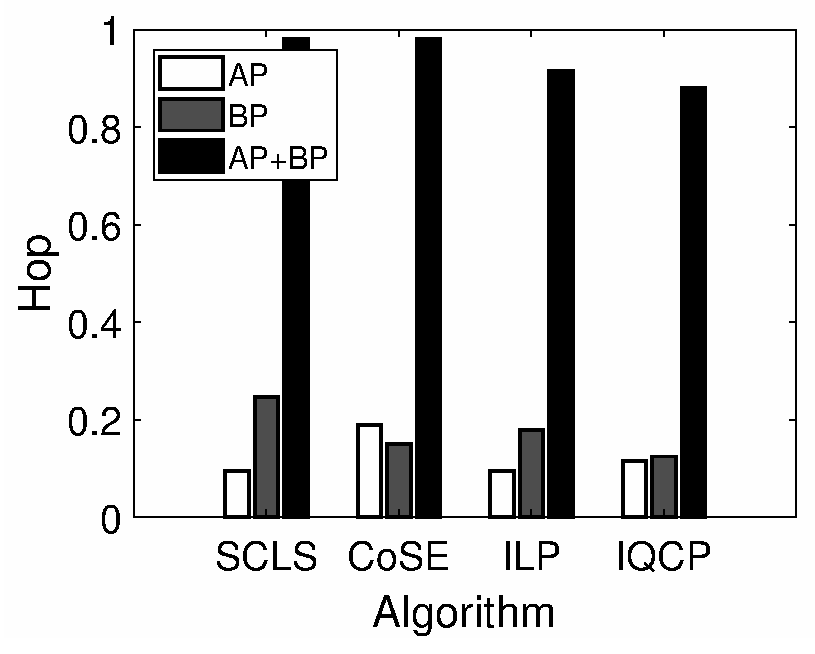
\includegraphics[width=.25\textwidth]{franz/hop.eps}
%  \caption{Path hop}\label{fig:normalization hop}
%\end{center}
% \includegraphics[width=.25\textwidth]{franz/runtime}\\
%  \caption{Runtime}\label{fig:normalization runtime}
%\end{figure*}

\begin{figure*}[tp]
\centering
\begin{minipage}[t]{0.3\linewidth}
\centering
\includegraphics[width=2.25in]{franz/weight}
\caption{Path weight}
\label{fig:normalization weitgh sum}
\end{minipage}
\hfill
\begin{minipage}[t]{0.3\linewidth}
\centering
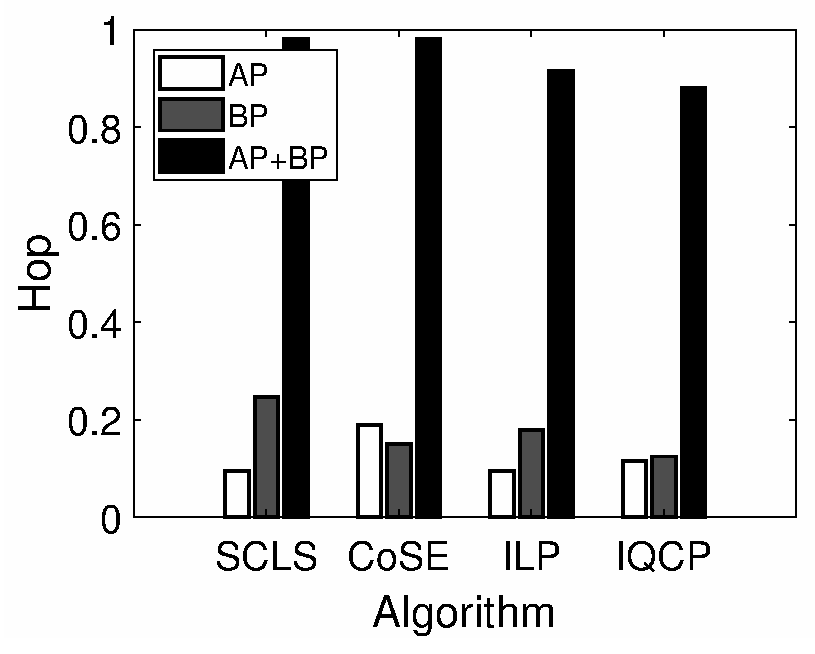
\includegraphics[width=2.25in]{franz/hop}
\caption{Path hop}
\label{fig:normalization hop}
\end{minipage}
\hfill
\begin{minipage}[t]{0.3\linewidth}
\centering
\includegraphics[width=2.25in]{franz/runtime}
\caption{Runtime}
\label{fig:normalization runtime}
\end{minipage}
\end{figure*}


\begin{figure*}[tp]
\centering
\begin{minipage}[t]{0.3\linewidth}
\centering
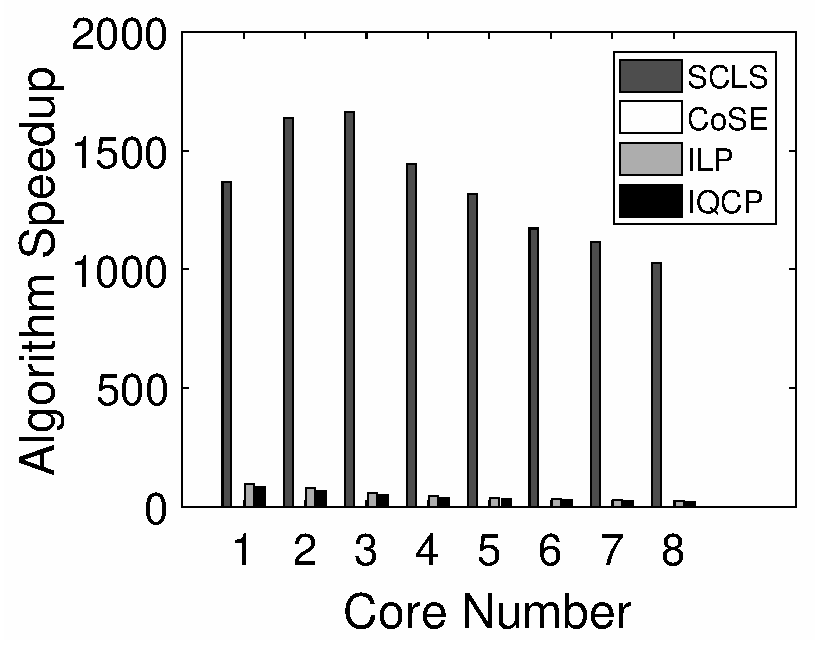
\includegraphics[width=2.25in]{franz/Multiple}
\caption{Algorithm speedup}
\label{fig:Multiple}
\end{minipage}
\hfill
\begin{minipage}[t]{0.3\linewidth}
\centering
\includegraphics[width=2.25in]{franz/speedup}
\caption{Core speedup}
\label{fig:Speedup}
\end{minipage}
\hfill
\begin{minipage}[t]{0.3\linewidth}
\centering
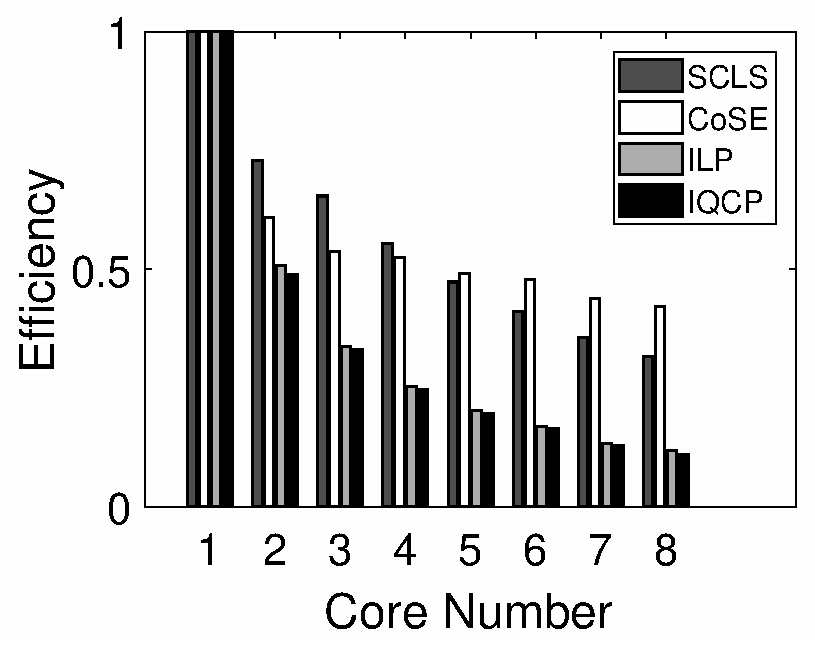
\includegraphics[width=2.25in]{franz/Efficiency}
\caption{Efficiency}
\label{fig:Efficiency}
\end{minipage}
\end{figure*}

%
%\begin{figure*}[htbp]
%\begin{minipage}[t]{0.35\linewidth}
%\centering
%\includegraphics[height=4.5cm,width=7.5cm]{franz/runtime.eps}
%\caption{one}
%\end{minipage}%
%\hfill
%\begin{minipage}[t]{0.5\linewidth}
%\centering
%\includegraphics[height=4.5cm,width=7.5cm]{franz/runtime.eps}
%\caption{two}
%\end{minipage}
%\end{figure*}

\subsubsection{Path Hop}
Fig.\ref{fig:normalization hop} shows the path hop of AP, BP, and the sum of both AP and BP. As all algorithms target to minimize the least path weight of the SRLG-disjoint path pair instead of the number of path hops, they have the same AP weight (Fig.\ref{fig:normalization weitgh sum}) even though they have different AP path hops (Fig.\ref{fig:normalization hop}). Although the AP weights under all algorithms are smaller than the BP weights in Fig.\ref{fig:normalization weitgh sum}, in Fig.\ref{fig:normalization hop}, the AP hops may not always be fewer than the BP hops.

%\begin{figure}
%  \centering
%  % Requires \usepackage{graphicx}
%  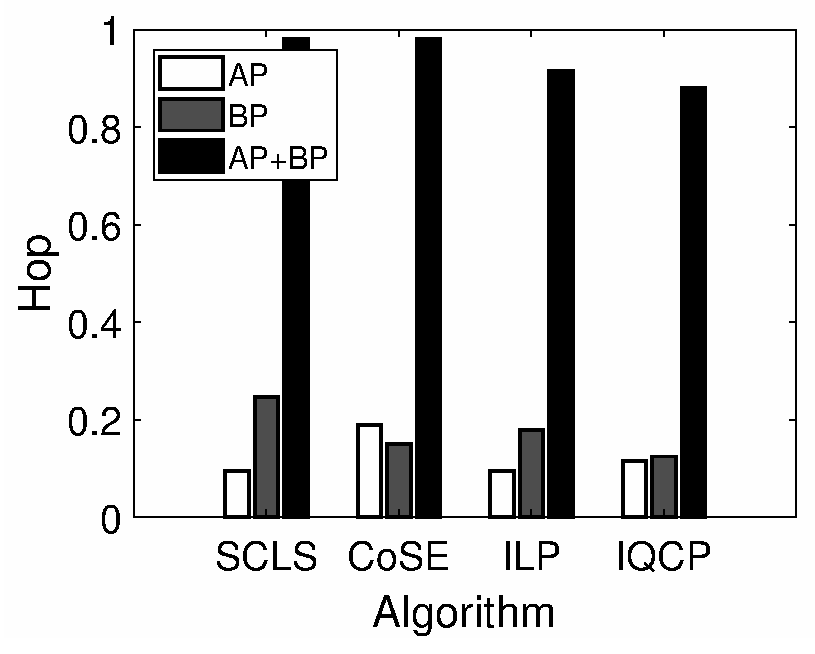
\includegraphics[width=2.35in]{franz/hop}\\
%  \caption{Path hop}\label{fig:normalization hop}
%\end{figure}

\subsubsection{Runtime}
\label{subsubsec:Runtime}
Fig.\ref{fig:normalization runtime} shows the run time under different algorithms by varying the number of CPU cores utilized.
As KSP, ILP, and IQCP are not parallel algorithms, the runtime of these algorithms under different number of cores is approximately equal. The runtime of our SCLS  and CoSE decreases with the increase of the number of processor cores because these two algorithms can partition the original problem into multiple sub-problems to execute in parallel and take advantage of the parallelism of the multi-core CPU to speed up the path searching process. Although CoSE is a parallel algorithm, the computation time is even larger than  ILP and IQCP. Some possible reasons include 1) the search process to find the conflicting SRLG set in CoSE  is not efficient; 2) As one SRLG usually includes multiple links, the partitioning of problem based on conflicting SRLG will introduce a large number of sub-problems to solve, which also results in a large computation cost.

%\begin{figure}
%  \centering
%  % Requires \usepackage{graphicx}
%  \includegraphics[width=2.35in]{franz/runtime}\\
%  \caption{Runtime}\label{fig:normalization runtime}
%\end{figure}

Different from CoSE, our SCLS looks for the set of conflicting links on an AP caught into the trap problem based on the min-cut theory in graph, and achieves the lowest time in Fig.\ref{fig:normalization runtime}. This demonstrates that our conflicting link set finding algorithm is efficient, and moreover our divide-and-conquer algorithm and intelligent AP searching process based on SRLG Conflicting Link Set can largely reduce the computation cost.

KSP is known as an effective algorithm to handle the trap problem. However, among all the algorithms implemented, the running time under KSP is the largest. A major problem of KSP is that after the current candidate AP fails the test (that is, it does not have a corresponding disjoint BP), the next candidate AP to be tested is selected solely based on the path length. In the 17 topologies we studied in the trace,  usually a large number of paths need to be tested in order to find a disjoint path pair (if it exists between a pair of nodes), thus KSP needs a large computation time.

Fig.\ref{fig:KSPproblem}  shows an example to illustrate why the KSP is extremely inefficient. In this graph, suppose SRLG conflicting link set is ${e_1,e_2}$, and the link weights of $e_1, e_2, e_3, e_4$ are much larger than other links. Then the first $K$ shortest weight paths from $s$ to $d$ will contain the shortest path segment $e_1,e_2$ denoted by the dotted line, which will further make the first shortest APs encounter the trap problem. To avoid the trap problem, $K$ have to be set as a large value, which brings a high time complexity to KSP. Different from KSP, when the shortest AP encounters the trap problem, we can quickly identify that \revtao{$\{e_1,e_2\}$} forms the SRLG conflicting link set, and then partition the original problem further into two subproblems $\mathcal{P}(\emptyset,\{e_1\})$ and \revtao{$\mathcal{P}(\{e_1\},\{e_2\})$} to execute in parallel on the multi-core CPU platform to quickly search for the SRLG disjoint path pair.

\begin{figure}[tp]
\centering
% Requires \usepackage{graphicx}
\includegraphics[width=3in]{franz/KSPproblem}
  \caption{An example to illustrate the inefficiency of KSP}
  \label{fig:KSPproblem}
\end{figure}

\subsubsection{Algorithm speedup}

In Fig.\ref{fig:Multiple}, we further compare their computation speeds. Specially, to calculate the speedup metric,
we use KSP as the baseline algorithm and set alg1 =KSP. Similar to the results in the Fig.\ref{fig:normalization runtime}, our SCLS achieves significantly larger speedup.

\subsubsection{Core speedup}

For the two parallel algorithms SCLS and CoSE, the core speedup   increases with the increase of the number of cores. %\del{Therefore, larger number of cores brings larger performance gain for these two parallel algorithms SCLS and CoSE.}
However, the increasing speed becomes smaller when the number of cores becomes larger and it incurs a higher cost to coordinate the process. Core speedup under algorithms KSP, ILP and IQCP is  approximately equal to 1 under any core number because they are not parallel algorithms. Among all algorithms, the core speedup of our SCLS is the largest, which demonstrates that our divide and conquer algorithm designed  based on the SRLG conflicting link set can bring the largest parallelism gain.

\note{How many paths pairs to search in your simulations. If you only search for one pair, then the sub=-problems may be lower than the number of cores, so multi core cannot be used.}
\subsubsection{Efficiency}
Efficiency is a measure of the overhead due to the parallelization. Programs with a high efficiency spend more time on useful work and less time on synchronization and communications. Similar to Fig.\ref{fig:Speedup}, with more cores involved, the efficiency value decreases  as a large core number brings more cost to coordinate the process. In Fig.\ref{fig:Efficiency}, the efficiency values of all algorithms decrease with the increase of the core number. Among all algorithms, the efficiency value of our SCLS is the largest under different core numbers, which demonstrates that our divide and conquer algorithm designed  based on the SRLG conflicting link set can bring the largest parallelism gain.



%\begin{figure}
%  \centering
%  % Requires \usepackage{graphicx}
%  \includegraphics[width=2.35in]{franz/runtime_nocose}\\
%  \caption{Normalization Runtime without CoSE value}\label{fig:normalization runtime_nocose}
%\end{figure}
%\subsubsection{Runtime's variance}
% As shown in Fig.\ref{fig:normalization runtime_var}.
%\begin{figure}
%  \centering
%  % Requires \usepackage{graphicx}
%  \includegraphics[width=2.35in]{franz/runtime_var}\\
%  \caption{Normalization Runtime Variance}\label{fig:normalization runtime_var}
%\end{figure}

%\subsubsection{Speed}
%The speedupSCLSte{bryant2003computer} of a parallel program is typically defined as
% \begin{equation}\label{equ:speed}
%   S_P=\frac{T_1}{T_p}
%\end{equation}
%where p is the number of processor cores and $T_k$ is the running time on k cores.Calculating the speedup of every processor cores in all algorithms in Fig.\ref{fig:Speedup} by the runtime of all algorithm from Fig.\ref{fig:normalization runtime}. The speedup value of CoSE increase with increasing the number of processor cores. The speedup value of CSLIE firstly increase then decrease because four cores is neck bottle of parallelism for CSLIE heuristic in this samples. The speedup value of other algorithm is affected slightly by the number of core processors.
%\begin{figure}
%  \centering
%  % Requires \usepackage{graphicx}
%  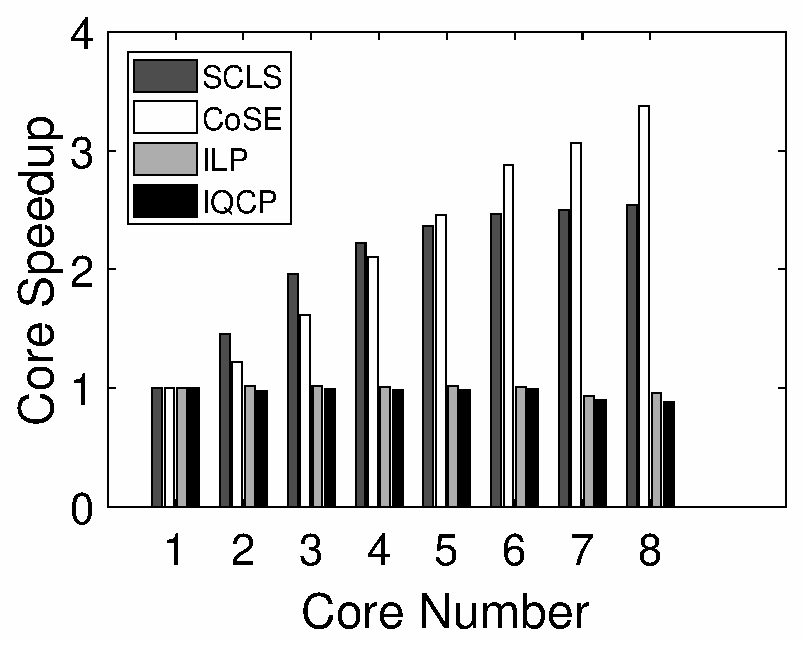
\includegraphics[width=2.35in]{franz/Speedup}\\
%  \caption{Speedup}\label{fig:Speedup}
%\end{figure}
%
%
%\subsubsection{Efficient}
%A related measureSCLSte{bryant2003computer} in Fig.\ref{fig:Efficiency}, known as efficiency, is defined as
%\begin{equation}\label{equ:efficient}
%  E_p=\frac{S_p}{p}=\frac{T_1}{pT_p}
%\end{equation}
%and is typically reported as a percentage in the range (0, 100]. Efficiency is a measure of the overhead due to parallelization. Programs with high efficiency are spending more time doing useful work and less time synchronizing and communicating than programs with low efficiency. Efficiet value of all algorithm decrease with the increase of core processors.
%\begin{figure}
%  \centering
%  % Requires \usepackage{graphicx}
%  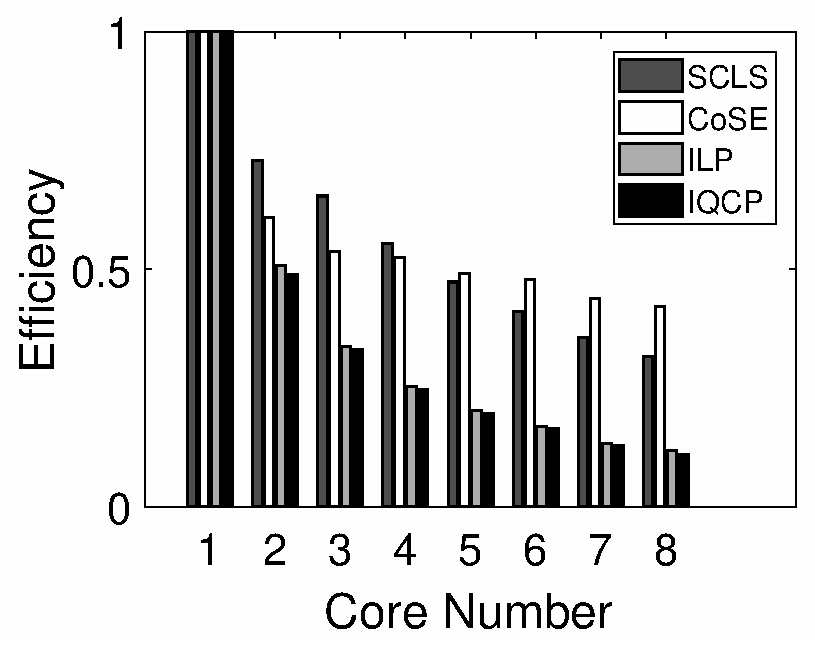
\includegraphics[width=2.35in]{franz/Efficiency}\\
%  \caption{Efficiency}\label{fig:Efficiency}
%\end{figure}
%\subsubsection{Multiple}
%The multiple's definition of parallel typically defined as
%\begin{equation}\label{equ:multiple}
%  M_n^x=\frac{T_n^{ILP}}{T_n^x}
%\end{equation}
%where x is algorithm such as CSLIE,CoSE,KSP ILP and IQCP. $T_n^x$ is the runtime of x algorithm in n processor cores. $T_n^{ILP}$ is the runtime of ILP in n processor cores. All algorithm compares with ILP runtime in Fig.\ref{fig:Multiple}

\section{conclusion}
\label{sec:conclusion}
%\del{In this paper, we have proved the Min-Min  SRLG-Disjoint routing problem is NP-complete.}
In this paper, we propose an efficient algorithm to solve the Min-Min  SRLG-Disjoint routing problem in the presence of the trap problem. To reduce the complexity of searching for the alternative pair, we propose a divide-and-conquer solution to partition the original Min-Min SRLG-Disjoint routing problem into multiple sub-problems based on a SRLG conflicting link set derived from the AP path encountering the trap problem. Our algorithm takes advantage of existing AP search results and parallel executions for significantly faster path finding.
We have conducted extensive simulations  using the topology trace  on a multi-core CPU platform. The simulation results demonstrate that our algorithm can outperform other approaches with higher routing performance while at a much higher search speed.
%\section*{Acknowledgment}
%%\end{spacing}
%The work is supported  by the  National Natural Science Foundation of China under Grant Nos.61572184, 61725206, 61472130, 61472131, and 61772191,  Hunan Provincial Natural Science Foundation of China under Grant No.2017JJ1010,  Science and Technology Key Projects of Hunan Province under Grant No.2015TP1004 and No.2016JC2012,  U.S. ONR N00014-17-1-2730, NSF ECCS 1408247, CNS 1526843, and ECCS 1731238.




%\input introduction
%\input related
%\input preniminaries
%\input problem
%\input overview
%\input conflict
%\input complete
%\input  srng
%\input performance
%\input conclusion
%\end{spacing}

\bibliographystyle{ieeetr}
\bibliography{reference}

\begin{IEEEbiography}[{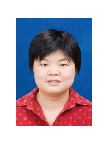
\includegraphics[width=1in,height=1.25in,clip,keepaspectratio]{fig/kunxie}}]{Kun Xie}
received  PhD
degree in computer application from Hunan University, Changsha, China,
in  2007. She worked as a postdoctoral fellow
in the department of computing in Hong Kong Polytechnic University from
2007.12 to 2010.2. She worked as a visiting researcher in the department
of electrical and computer engineering in state university of New York at
Stony Brook from 2012.9 to 2013.9. Her research interests include wireless network and mobile
computing, network management and control, cloud computing and mobile
cloud, and big data. She has published over 60 papers in major journals and conference proceedings
(including top journals IEEE/ACM TON, IEEE TMC, IEEE TC, IEEE TWC, IEEE TSC, and top conferences INFOCOM, ICDCS, SECON, IWQoS)
\end{IEEEbiography}
\begin{IEEEbiography}[{\includegraphics[width=1in,height=1.25in,clip,keepaspectratio]{fig/taoheng}}]{Heng Tao}
 is now a master student in the department of electrical and computer engineering in state university of New York at
Stony Brook. His research interests include SDN routing and bloom filter.
\end{IEEEbiography}
\begin{IEEEbiography}[{\includegraphics[width=1in,height=1.25in,clip,keepaspectratio]{fig/xinwang}}]{Xin Wang}
 received the Ph.D. degree in electrical and computer engineering from Columbia University, New York, NY.
She is currently an Associate Professor in the Department of Electrical and Computer Engineering of the State University of New York at Stony Brook, Stony Brook, NY. Before joining Stony Brook, she was a Member of Technical Staff in the area of mobile and wireless networking at Bell Labs Research, Lucent Technologies, New Jersey, and an Assistant Professor in the Department of Computer Science and Engineering of the State University of New York at Buffalo, Buffalo, NY. Her research interests include algorithm and protocol design in wireless networks and communications, mobile and distributed computing, as well as networked sensing and detection. She has served in executive committee and technical committee of numerous conferences and funding review panels, and served as the associate editor of IEEE Transactions on Mobile Computing. Dr. Wang achieved the NSF career award in 2005, and ONR challenge award in 2010.
\end{IEEEbiography}




%\begin{IEEEbiography}[{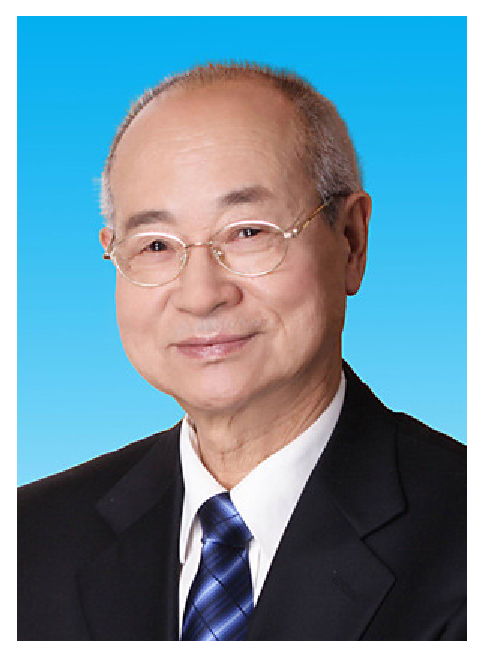
\includegraphics[width=1in,height=1.25in,clip,keepaspectratio]{fig/minyinghua}}]{Yinghua Min} graduated from mathematics department of Jilin university, Changchun, China in 1962, and completed his graduate study in electrical engineering at China Academy of Railway Sciences, Beijing in 1966, although no degree was issued at that time in P.R.China.  He has visited Stanford and other universities in the US for years since 1981.  He is now a professor of Computer science at Institute of Computing Technology, Chinese Academy of Sciences, Beijing, the associate editor-in-chief of 鈥淛ournal of Computer Science and Technology? Honored Chair of technical committee on fault-tolerant computing, China Computer Federation.  He is also a member of the expert committee of the SOC project for the National Natural Science Foundation of China.  He published 230 technical papers, and 4 books, and received the Natural Science award three times from the Chinese Academy of Sciences.  He served as general chairs and program chairs for a number of IEEE symposia and workshops. He is now Co-Chair of the Dragon Star program, a program for US professors to help the People鈥檚 Republic of China (PRC) to improve its graduate education in Computer Science and Engineering. He is a Fellow of IEEE, a member of ACM, and a Golden Core Member of IEEE Computer Society.  His current research interests include electronic testing, dependable computing, and networking.
%\end{IEEEbiography}

%\begin{IEEEbiography}[{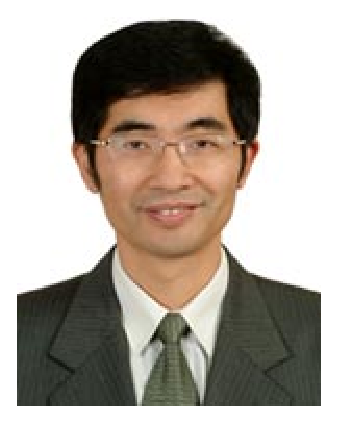
\includegraphics[width=1in,height=1.25in,clip,keepaspectratio]{fig/dafangzhang}}]{Dafang Zhang} received Ph.D. degree in Application Mathematics in Hunan University, Changsha, China, in 1997. He is currently a professor with Hunan University, Changsha, China. His research interests include packet processing, Internet measurement, wireless network and mobile computing, and big data.
%\end{IEEEbiography}

%\begin{IEEEbiography}[{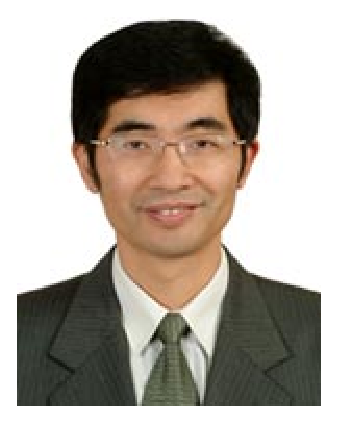
\includegraphics[width=1in,height=1.25in,clip,keepaspectratio]{fig/dafangzhang}}]{Dafang Zhang} received Ph.D. degree in Application Mathematics in Hunan University, Changsha, China, in 1997. He is currently a professor with Hunan University, Changsha, China. His research interests include packet processing, Internet measurement, wireless network and mobile computing, and big data.
%\end{IEEEbiography}


%\begin{IEEEbiography}[{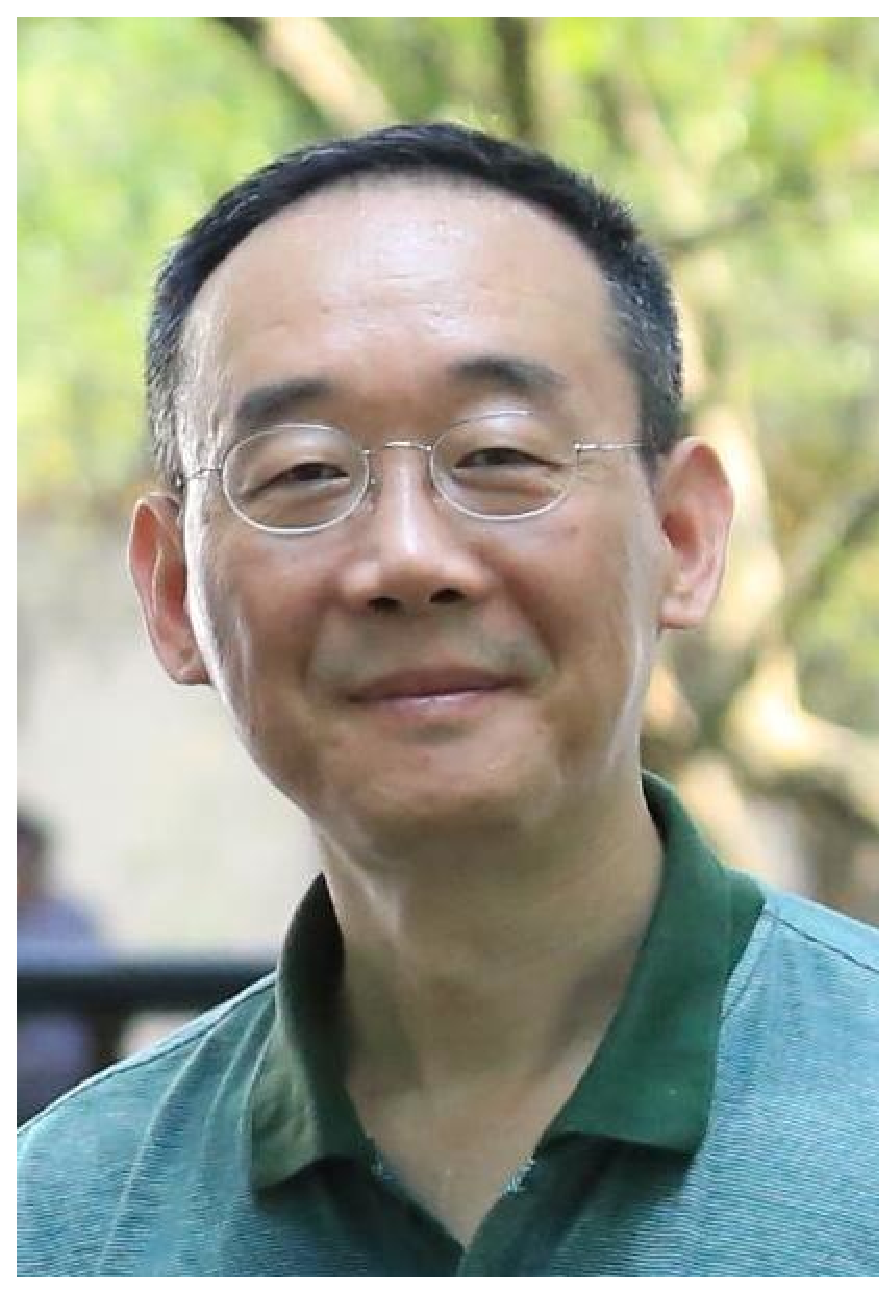
\includegraphics[width=1in,height=1.25in,clip,keepaspectratio]{fig/KeqinLi}}]{Keqin Li} is a SUNY Distinguished Professor of computer science.His current research interests include parallel computing and high-performance computing,
%distributed computing,energy-efficient computing and communication,heterogeneous computing systems,cloud computing,big data computing,CPU-GPU hybrid and cooperative computing,multicore computing,storage and file systems,wireless communication networks,sensor networks,peer-to-peer file sharing systems,mobile computing,service computing,Internet of things and cyber-physical systems.He has published over 400 journal articles, book chapters, and refereed conference papers,and has received several best paper awards.He is currently or has served on the editorial boards of
%{\em IEEE Transactions on Parallel and Distributed Systems},{\em IEEE Transactions on Computers},{\em IEEE Transactions on Cloud Computing},
%{\em Journal of Parallel and Distributed Computing}.He is an IEEE Fellow.
%\end{IEEEbiography}
%\vspace{-30pt}

\begin{IEEEbiography}[{
\includegraphics[width=1in,height=1.25in,clip,keepaspectratio]{fig/gaogangxie}}]{Gaogang Xie}
received his B.S. degree in Physics, M.S. degree and Ph.D. degree in computer science all from Hunan University respectively in 1996, 1999 and 2002. He is currently a Professor and Director of Network Technology Research Center with the Institute of Computing Technology (ICT), Chinese Academy of Sciences (CAS), Beijing, China. His research interests include Internet architecture, packet processing and forwarding, and Internet measurement.
\end{IEEEbiography}

\begin{IEEEbiography}[{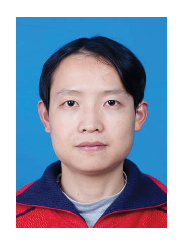
\includegraphics[width=1in,height=1.25in,clip,keepaspectratio]{fig/jigangwen}}]{Jigang Wen}
received PhD degrees in computer application from Hunan University, China, in 2011. He worked as a research assistant in the department of computing in Hong Kong Polytechnic University from 2008 to 2010. He is now a postdoctoral fellow
in Institute of Computing Technology, Chinese Academy of Science, China. His research interests include wireless network and mobile computing, high speed network measurement and management.
\end{IEEEbiography}
\end{document}
%\section{EeVSN Formulation}
After designing an EVN, in this section, we also formulate
its embedding problem as an MILP fitting for both FD-EVN
and FI-EVN embedding, since the difference between them in
embedding approach could be reconciled by a general resources
sharing constraint. More details would be elaborated in the following
part.

with respect to the node embedding, we
have the assumption that all the virtual nodes in EVN should be
mapped on physically isolated substrate nodes.

different node failure scenarios.
Thus, rather than solving the link embedding problem based
on the multi-commodity flow LP, we need consider the resource
sharing issues, which is computational intractable. As a result,
heuristic algorithms with acceptable computation complexity.


%\input{EeVSNDesign}
